% !TEX root = main.tex
% Tipo di documento. L'uso di twoside implica che i capitoli inizino sempre con la prima pagina a sinistra, eventualmente lasciando una pagina vuota nel capitolo precedente. Se questa cosa è fastidiosa, è possibile rimuoverlo. 
\documentclass[a4paper, twoside,openright]{report}
% \documentclass[a4paper,openright]{report}

% \usepackage{fancyhdr}
% \pagestyle{fancy}
% \fancyhf{}
% \lhead{\rightmark}
% \rhead{\textbf{\thepage}}
% % \fancyfoot{}
% \setlength{\headheight}{12.5pt}
% Rimuove il numero di pagina all'inizio dei capitoli
% \fancypagestyle{plain}{
%   \fancyfoot{}
%   \fancyhead{}
%   \renewcommand{\headrulewidth}{0pt}
% }


\usepackage{graphicx} % Required for inserting images
\setkeys{Gin}{width=0.6\columnwidth}

\usepackage[utf8]{inputenc}

\usepackage{hyperref}
\usepackage{adjustbox}

\usepackage{wrapfig}

\usepackage{enumitem}
\renewcommand{\labelitemi}{$\diamond$}
\renewcommand{\labelitemiii}{$\circ$}
\setlist[enumerate,2]{label=\roman*.}
\setlist[enumerate,3]{label=(\alph*)}

\setitemize{noitemsep}
\setenumerate{noitemsep}
\setlist{noitemsep}

\usepackage{paracol}
\usepackage{multicol}
\usepackage{booktabs}


\usepackage{geometry}

\usepackage{color}

\usepackage{listings}
% \usepackage{minted}

\usepackage{amsmath}
\usepackage{amssymb}
\usepackage{amsfonts}
\usepackage{mathtools}
\usepackage{bm}
\usepackage{nicefrac, xfrac}

\usepackage{wasysym}

% Uso dei colori
\usepackage[dvipsnames,table,xcdraw]{xcolor}
\usepackage{colortbl}
\usepackage{rotating}
\usepackage{adjustbox}

\usepackage{multirow}
\usepackage{booktabs}
\usepackage{makecell}


\usepackage{tikz}
\usetikzlibrary{automata, arrows,bending}
\usetikzlibrary{positioning}
\usetikzlibrary{shapes.geometric}
\usepackage{parskip}
\usepackage{changepage}

\usepackage{soul}
\usepackage{cancel}

% This are needed because the correct double quotes would be ``'' or ``",
% but i've always written "text"
% TODO - check whether this affects listing environment
% \usepackage [english]{babel}
% \usepackage [autostyle, english = american]{csquotes}
% \MakeOuterQuote{"}

\geometry{margin=0.6in}

\setlist[description]{itemsep=0em,topsep=0.5em,parsep=0em}
\setlist[itemize]{itemsep=0em,topsep=0pt}
\setlist[enumerate]{itemsep=0em,topsep=0pt}

\hypersetup{
    colorlinks=true,
    linkcolor=black,
    filecolor=mauve,
    urlcolor=blue,
}

\definecolor{gray}{gray}{0.3}
\definecolor{verylightgray}{gray}{0.95}
\definecolor{blue}{rgb}{0,0,1}
\definecolor{mauve}{rgb}{0.58,0,0.82}
\definecolor{darkred}{rgb}{0.3,0,0}
\definecolor{darkgreen}{rgb}{0,0.3,0}
\definecolor{darkgray}{gray}{0.15}



\newenvironment{notes}{
\par
\color{gray}
\small}

\newcommand{\note}[1]{\begin{notes}{#1}\end{notes}}
\newcommand{\nl}[0]{\parskip = \baselineskip}
\newcommand{\lst}[1]{\lstinline{#1}}
\newcommand{\ra}{\xrightarrow{\hspace*{2em}}}
\newcommand{\ns}{\setlength{\parskip}{0em}}

\newlength{\currentparindent}
\newcommand{\labelitemize}[2]{
\setlength{\currentparindent}{\parindent}
\setlength{\parindent}{0pt}

\begin{minipage}{0em} % Adjust the width as needed
    \makebox[0em][c]{\rotatebox{90}{\small #1}}
\end{minipage}
\begin{minipage}{\dimexpr\columnwidth-1cm\relax}
    #2
\end{minipage}
\setlength{\parindent}{\currentparindent}
}
\newcommand{\colfill}{\vspace{\fill}}

\newcommand{\framed}[1]{
\begin{center}
\fbox{
    \begin{minipage}{0.8\columnwidth}
        #1
    \end{minipage}
}
\end{center}}

\newcommand{\framedt}[2]{
\begin{center}
\fbox{
    \begin{minipage}{0.8\columnwidth}
        \vspace*{1em}
        \begin{center}
            \textbf{\ul{#1}}
        \end{center}
        \nl
        #2
    \end{minipage}
}
\end{center}}

\newcommand{\proscons}[4]{
    \begin{paracol}{2}
        \labelitemize{\color{darkgreen}\ul{\textit{#1}}}{
           \color{darkgreen}
           #3
        }
        \switchcolumn
        \labelitemize{\color{darkred}\ul{\textit{#2}}}{
           \color{darkred}
           #4
        }
     \end{paracol}
}

\newcommand\hcancel[2][black]{\setbox0=\hbox{$#2$}%
\rlap{\raisebox{.45\ht0}{\textcolor{#1}{\rule{\wd0}{1pt}}}}#2} 


\lstset{frame=false,
 showstringspaces=false,
 breaklines=true;
 columns=flexible,
 basicstyle={\small\ttfamily},
 keywordstyle=\color{blue},
 commentstyle=\color{darkgreen},
 stringstyle=\color{mauve}
 tabsize=3
}

\newtheorem{definition}{Definition}[chapter]
\newtheorem{theorem}{Theorem}[chapter]

\usepackage{fancyhdr}
% \usepackage{nameref,autoref}

\pagestyle{fancy}
\fancyhf{}
\fancyhead[LE,RO]{\thepage} % Page number on Outer side of header on each page
\fancyhead[LO]{\leftmark} % section title on Left side of header on Odd pages
\fancyhead[RE]{\rightmark} % subection title on Right side of header on Even pages
\fancyfoot{}
\renewcommand{\headrulewidth}{0.4pt} % Width of line under the header
% \setcounter{secnumdepth}{2} % Depth of sectioning commands to include in the table of contents

% Rimuove il numero di pagina all'inizio dei capitoli
\fancypagestyle{plain}{
  \fancyfoot{}
  \fancyhead{}
  \renewcommand{\headrulewidth}{0pt}
}

\usepackage{emptypage}



\title{Data Mining - Appunti}
\author{Francesco Lorenzoni}
\date{Febrero 2025}


\makeatletter
\renewcommand{\l@section}{\@dottedtocline{1}{1.5em}{2.6em}}
\renewcommand{\l@subsection}{\@dottedtocline{2}{2.5em}{3.6em}}
\renewcommand{\l@subsubsection}{\@dottedtocline{3}{3.5em}{4.5em}}
\makeatother
\mtcsettitle{parttoc}{Contents of this Part} % Set the title for the part TOC


\begin{document}
\doparttoc[n]

\maketitle
\tableofcontents

\part{Introduction to Data Mining}
\parttoc
\chapter{Práctica 4 y 5}

% No necesario con minted (se especifica al usar el entorno)
\lstset{language=python}

% Preface
% \note{Soy un estudiante italiano en Erasmus. Hablo español bastante bien, pero me resulta más natural escribir en inglés; sin embargo, decidí escribir en español para practicar, con la ayuda de algunos traductores cuando era necesario. Si hay algo mal escrito o poco claro, estoy a disposición para cualquier aclaración.}

\section{Ejercicios 1/2/3 - \texttt{sin\_vocales}}

\subsection{Ejercicio 1 - Función inicial}
\begin{lstlisting}[captionpos=b,caption={Función inicial}]
   def sin_vocales (s):
      """
      devuelve el argumento s sin vocales
      """
      vocales = 'aeiou'
      s_sinVocales = ' '
      for ch in s:
         pos = vocales.find(ch)
         if pos == -1: #ch no es vocal
            s_sinVocales = s_sinVocales + ch
      return s_sinVocales
\end{lstlisting}

Esta es la función inicial que se nos ha dado, y que parece funcionar, pero solo con pruebas demasiado sencillas.

\subsection{Ejercicio 2 - Prueba de la función}

Abajo en el código \ref{code:pruebas}, después de la discusión de los dos errores encontrados, hay la función	de prueba completa \lstinline{test_sin_vocales()} que comprueba la función \lstinline{sin_vocales(s)}. 


\begin{paracol}{2}
   \colfill
   El primero error en la función dada \lstinline{sin_vocales(s)} es que \ul{no se tiene cuenta de las \textbf{mayúsculas} y \textbf{minúsculas}}. Por lo tanto, la función no elimina las vocales mayúsculas. Para solucionarlo, es suficiente añadir a la lista de vocales la versión mayúscula de cada vocal.
   \colfill

   \switchcolumn

   \begin{lstlisting}
def test_sin_vocales():
   s = "el agua esta mojada"
   exp = "l g st mjd"
   assert sin_vocales(s) == exp

   ...
      
   s = "El AgUe eStA mOjAdA"
   exp = "l g St mjd"
   assert sin_vocales(s) == exp
   \end{lstlisting}
\end{paracol}

\begin{lstlisting}[captionpos=b,caption={\lstinline|sin_vocales()| con vocales mayúsculas}, label={code:sin_vocales1}]
   def sin_vocales (s:str):
      vocales = 'aeiouAEIOU'
      s_sinVocales = ''
      for ch in s:
         pos = vocales.find(ch)
         if pos == -1: #ch no es vocal
            s_sinVocales = s_sinVocales + ch
      return s_sinVocales
\end{lstlisting}

\newpage
\begin{paracol}{2}
   \colfill
   El segundo error es que la función \ul{no tiene cuenta de los \textbf{acentos}}. Por lo tanto, la función no elimina las vocales acentuadas.
   \begin{lstlisting}
   assert sin_vocales("áÉíÓú") == "" # falla
   \end{lstlisting}
   Para solucionarlo, es suficiente añadir a la lista de vocales la versión acentuada de cada vocal.

   \begin{lstlisting}
   vocales = 'aeiouAEIOUáéíóúàèìòùäëïöüâê
   îôûÁÉÍÓÚÀÈÌÒÙÄËÏÖÜÂÊÎÔÛãõÃÕ'
   \end{lstlisting}

   Esta solución no parece muy elegante, ya que la lista de vocales se vuelve muy larga. Buscando sobre el internet he visto que una solución más elegante sería usar una expresión regular para eliminar todas las vocales, acentuadas o no. Para ello, se puede usar el módulo \lstinline{re} de Python, junto con \lstinline{unicodedata}, como se muestra en el código a la derecha.
   \colfill

   \switchcolumn
   \colfill
   \begin{lstlisting}[label={code:unicodedata},captionpos=b,caption={Código para eliminar vocales y diacríticos que utiliza \lstinline{unicodedata}}]
import unicodedata
import re

def sin_vocales(s):
   # Normaliza el texto separando los caracteres básicos de sus diacríticos
   s_norm = unicodedata.normalize('NFD', s)
   # Elimina todas las vocales base y los diacríticos
   s_sin_vocales = re.sub(r'[aeiouAEIOU\u0300-\u036f]', '', s_norm)
   return s_sin_vocales
   \end{lstlisting}
   \colfill
\end{paracol}

\vspace{2em}

\begin{lstlisting}[captionpos=b,caption={Pruebas que he escrito}, label={code:pruebas}]
def test_sin_vocales():
   s = "el agua esta mojada"
   exp = "l g st mjd"
   assert sin_vocales(s) == exp
   s = "aieou"
   exp = ""
   assert sin_vocales(s) == exp
   s = "123greee"
   exp = "123gr"
   assert sin_vocales(s) == exp
   s = "El AgUe eStA mOjAdA"
   exp = "l g St mjd"
   assert sin_vocales(s) == exp
   s = "àéíóú"
   exp = ""
   assert sin_vocales(s) == exp
   s = "are you ok?"
   exp = "r y k?"
   assert sin_vocales(s) == exp
   s = ""
   exp = ""
   assert sin_vocales(s) == exp
   s = "A"
   exp = ""
   assert sin_vocales(s) == exp
   
\end{lstlisting}
\subsection{Ejercicio 3/4 - Corregir la función y añadir pruebas}

\begin{lstlisting}[captionpos=b,caption={\lstinline|sin_vocales()| corregida}, label={code:sin_vocales}]
   def sin_vocales (s:str):
      vocales = 'aeiouAEIOUáéíóúàèìòùäëïöüâêîôûÁÉÍÓÚÀÈÌÒÙÄËÏÖÜÂÊÎÔÛãõÃÕ'
      s_sinVocales = ''
      for ch in s:
         pos = vocales.find(ch)
         if pos == -1: #ch no es vocal
            s_sinVocales = s_sinVocales + ch
      return s_sinVocales
\end{lstlisting}

Para evitar el uso del paquete adicional \lstinline{unicodedata}, he preferido utilizar simplemente listas de vocales que incluyen también las vocales acentuadas.

He añadido al fichero \texttt{.py} la función que nos ha dado en el ejercicio, per controllare che anche quei test passassero.

\newpage
\section{Ejercicio 5 - \texttt{cantidad\_numeros}}
\begin{lstlisting}[captionpos=b,caption={Solución sencilla}]
def cantidad_numeros_sencilla(s: str):
   """
   Esta función recibe una cadena de texto y devuelve la cantidad de números que contiene.
   N.B. números, no digitos!
   """
   return len(re.findall(r'\d+', s))
\end{lstlisting}

Esta primera solución funciona y es concisa, pero no tiene en cuenta los números decimales (como $12.34$) y las notaciones científicas (como $12\cdot 10^6$ o $10^{-2}$). 
Para solucionarlo, es necesario modificar la expresión regular para que también considere estos casos.

\begin{lstlisting}[captionpos=b,caption={Solución que incluye números decimales y notaciones científicas}]
      
def cantidad_numeros(s: str):
   """
   Esta función recibe una cadena de texto y devuelve la cantidad de números que contiene.
   
   Números decimales (como 12.34) y notaciones científicas (como 12*10^6 o 10^(-2)) son considerados números.
   """
   # Identificar números decimales (como 12.34)
   decimal_pattern = r'-?\d+\.\d+'
   decimal_matches = re.findall(decimal_pattern, s)
   
   # Eliminar los números decimales ya encontrados para evitar contar dos veces
   for match in decimal_matches:
       s = s.replace(match, ' ', 1)
   
   # Identificar notaciones científicas (como 12*10^6 o 10^(-2))
   scientific_pattern = r'\d+\*10\^\(?\-?\d+\)?'
   scientific_matches = re.findall(scientific_pattern, s)
   
   # Eliminar las notaciones científicas de la cadena
   for match in scientific_matches:
       s = s.replace(match, ' ', 1)
   
   # Encontrar los números restantes (enteros)
   # Modificamos el patrón para capturar secuencias de dígitos en cualquier contexto
   remaining_pattern = r'\d+'
   remaining_matches = re.findall(remaining_pattern, s)
   
   # Contar el total de números encontrados
   return len(decimal_matches) + len(scientific_matches) + len(remaining_matches)
\end{lstlisting}

\newpage
\begin{paracol}{2}
   
   \begin{lstlisting}[captionpos=b,caption={Mis pruebas para \lstinline|cantidad_numeros()|}, label={code:cantidad_numeros}]
def test_cantidad_numeros():
   s = "12 356 53333"
   assert cantidad_numeros(s) == 3
   s = "asfa432asf23"
   assert cantidad_numeros(s) == 2
   s = ""
   assert cantidad_numeros(s) == 0
   s = "1"
   assert cantidad_numeros(s) == 1
   s = "fwgds"
   assert cantidad_numeros(s) == 0
   s = "1 fhsdSGG 4"
   assert cantidad_numeros(s) == 2
   s = "-12 + 34 -12-133 "
   assert cantidad_numeros(s) == 4
   s = "12.34 56.78"
   assert cantidad_numeros(s) == 2
   s = "12*10^6"
   assert cantidad_numeros(s) == 1
   s = "23*10^(-2)"
   assert cantidad_numeros(s) == 1
   s = "23*10^(64) + 12.34"
   assert cantidad_numeros(s) == 2
   s = "asgre23*10^(-2)asfg10^2"
   assert cantidad_numeros(s) == 2
   s = "asgre23*10^(-2)asfg10^2agr12.34"
   assert cantidad_numeros(s) == 3
   \end{lstlisting}

   \switchcolumn

   \begin{lstlisting}[captionpos=b,caption={Pruebas ordenadas como estan en el documiento}, label={code:cantidad_numeros2}]
def test_cantidad_numeros_doc():
   # Varios números en la cadena
   s = "un 1, un 201 y 2 unos"   
   assert cantidad_numeros(s) == 3
   # Sin números en la cadena
   s = "sin numeros"   
   assert cantidad_numeros(s) == 0
   # Un solo número en la cadena
   s = "2345543"    
   assert cantidad_numeros(s) == 1
   # Diferentes longitudes de números
   s = "1 22 333 4444 55555"    
   assert cantidad_numeros(s) == 5
   # Números separados por espacios
   s = "123 456 789"    
   assert cantidad_numeros(s) == 3
   # Números separados por comas
   s = "12,34,56,78"    
   assert cantidad_numeros(s) == 4
   # Números rodeados de texto
   s = "numero123numero456numero"   
   assert cantidad_numeros(s) == 2
   # Una cadena continua de números
   s = "123456789"   
   assert cantidad_numeros(s) == 1
   # Números al inicio y al final
   s = "1 starting and ending 2"    
   assert cantidad_numeros(s) == 2
   # Número al final 
   s = "ending with number 5"   
   assert cantidad_numeros(s) == 1
   # Números en una cadena simple
   s = "3 6 9"   
   assert cantidad_numeros(s) == 3
   # Sin números en la cadena
   s = "sinnumeros"    
   assert cantidad_numeros(s) == 0
   # Números mezclados con texto
   s = "123unnumero456"   
   assert cantidad_numeros(s) == 2
   # Números negativos
   s = "-5 10 -15"  
   assert cantidad_numeros(s) == 3
   \end{lstlisting}
\end{paracol}

\newpage
\section{Ejercicio 6 - \texttt{sin\_vocales} con prueba parametrizada}

\begin{lstlisting}
@pytest.mark.parametrize ("entrada , salida_esperada " ,[
   ("El agua esta mojada", "l g st mjd"),
   ("mojada bañando en el agua", "mjd bñnd n l g"),
   ("ahora termina bien", "hr trmn bn"),
   ("", ""),
   ("a", ""),
   ("m", "m"),
   ("unstringsinespacios", "nstrngsnspcs"),
   ("MAYUSculas FUNCIOnaN", "MYScls FNCnN"),
   ("krt yhgf dwpq", "krt yhgf dwpq"),
   ("aeoiuuuoiea", ""),
   ("disco de los 80", "dsc d ls 80"),
   ("signos como ? y ! y ¡", "sgns cm ? y ! y ¡"),
   ("ábc élla ó", "bc ll "),
   ("Óm tambien mayÚsculÁs", "m tmbn myscls")
   ])

def test_sin_vocales_parametrizado(entrada, salida_esperada):
   """
   testea la función sin_vocales
   """
   assert sin_vocales (entrada) == salida_esperada
\end{lstlisting}

Esta es una forma alternativa de escribir los test, que permite de parametrizar la función driver de test.

En comparación con el test set anterior del pdf, hemos añadido pruebas que incluyen vocales con acento. La función \lstinline|sin_vocales| no va a cambiar porque ya había tenido en cuenta los acentos en el ejercicio anterior.




\chapter{Tarea 2}

% TAREA 2.

%     Visualiza el siguiente vídeo:

% https://www.google.com/search?client=firefox-b-d&q=Kaspersky+Industrial+CyberSecurity+demonstration+for+Energy+sector+-+Bing+video+#fpstate=ive&vld=cid:fc74c561,vid:7LNtjWx17mA,st:0


\framedt{Tarea a realizar}{

   Visualiza el siguiente vídeo:
   \href{
      https://www.youtube.com/watch?v=7LNtjWx17mA
   }{youtube.com/watch?v=7LNtjWx17mA}
   
   \begin{itemize}
   	\item Identifica en la red industrial los componentes físicos, ciberfísicos, y ciber
	\item Identifica los tipos de ataque que se describen en el vídeo, y explica brevemente como piensas que se podrían implementar.
	\item Explica cómo plantea la solución de Kaspersky en el vídeo la defensa frente a los posibles ataques.
   \end{itemize}
}


%     Contesta a las siguientes preguntas:

%     Identifica en la red industrial que se describe en el vídeo:

% a. Lo componentes físicos

% b. Los componentes ciberfísicos

% c. Los componentes ciber

%     Identifica los tipos de ataque que se describen en el vídeo, y explica brevemente como piensas que se podrían implementar.

%     Explica cómo plantea la solución de Kaspersky en el vídeo la defensa frente a los posibles ataques.

\begin{figure}[htbp]
   \centering
   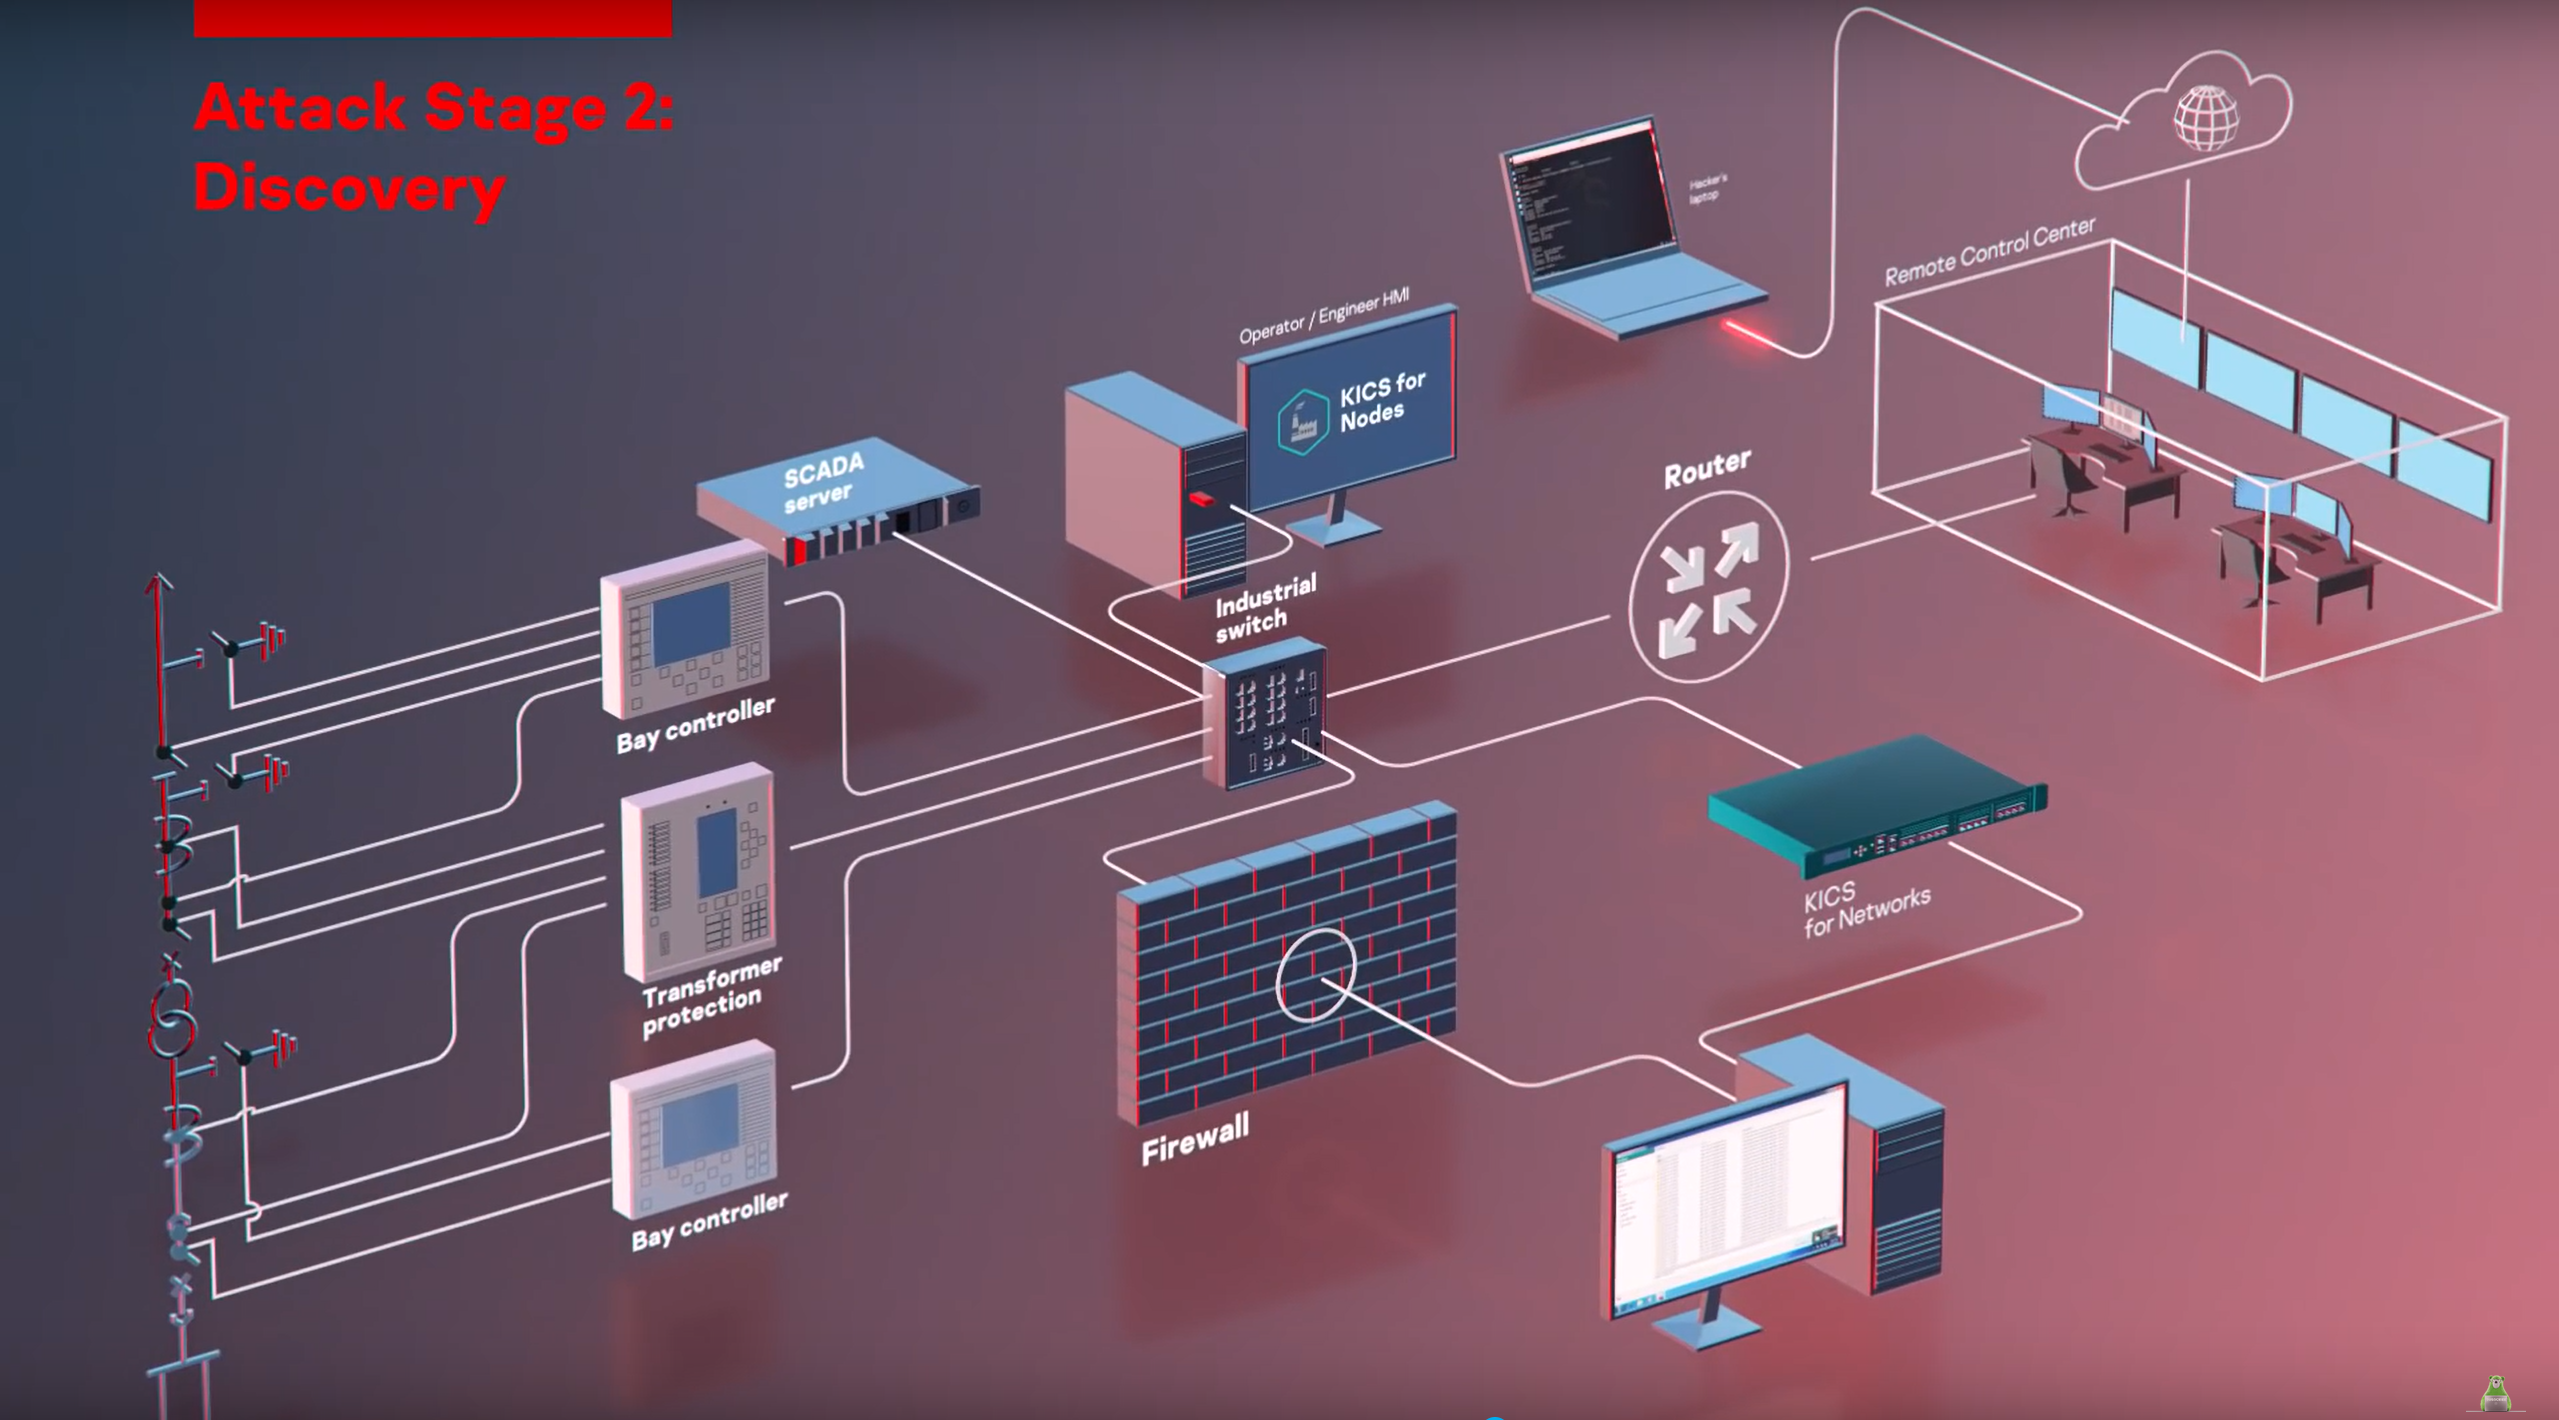
\includegraphics{images/ICSscenario.png}
   \caption{Escenario representado en el vídeo}
   \label{fig:ICSscenario}
\end{figure}


\section{Componentes de la red industrial}

\begin{itemize}
   \item \textbf{Componentes físicos:}
   \begin{itemize}
      \item 100kv high-voltage incoming line
      \item Power transformer
      \item 10kV bus feeder
      \item Primary switching equipment
   \end{itemize}
   \item \textbf{Componentes ciberfísicos:}
   \begin{itemize}
      \item transformer protection
      \item 2 bay controllers
      \item Industrial Ethernet switch
   \end{itemize}
   \item \textbf{Componentes ciber:}
   \begin{itemize}
      \item Kaspersky Industrial CyberSecurity
      \begin{itemize}
         \item \textsc{KICS} for Nodes - Endpoint Protection
         \item \textsc{KICS} for Network - Anomaly and Breach Protection
         \item Centralized security management
         \item Kasperky Security Center - Manager installed on nodes
      \end{itemize}
      \item Router
      \item Firewall
      \item Remote Control Center tools
      \item SCADA server
   \end{itemize}
\end{itemize}

\subsection{Kaspersky Industrial CyberSecurity (\textsc{KICS})}
% Software / hardware / virtual appliance
\begin{paracol}{2}
   
   Las ---``claimed''--- features de \textsc{KICS} son las siguientes:
   \begin{itemize}
	\item Passive traffic analysis
	\item No influence on network stability
	\item Detection of:
	\begin{itemize}
      \item Unauthorized network access
      \item Cyberattacks and intrusions
      \item Unauthorized commands to industrial equipment
      \item Technological parameters anomalies:
      \begin{itemize}
         \item Rules based
	      \item Machine learning
      \end{itemize}
      \item Assets and its parameters
      \item Abnormal dataflow on network map
   \end{itemize}
\end{itemize}

\switchcolumn

\colfill
\begin{figure}[htbp]
   \centering
   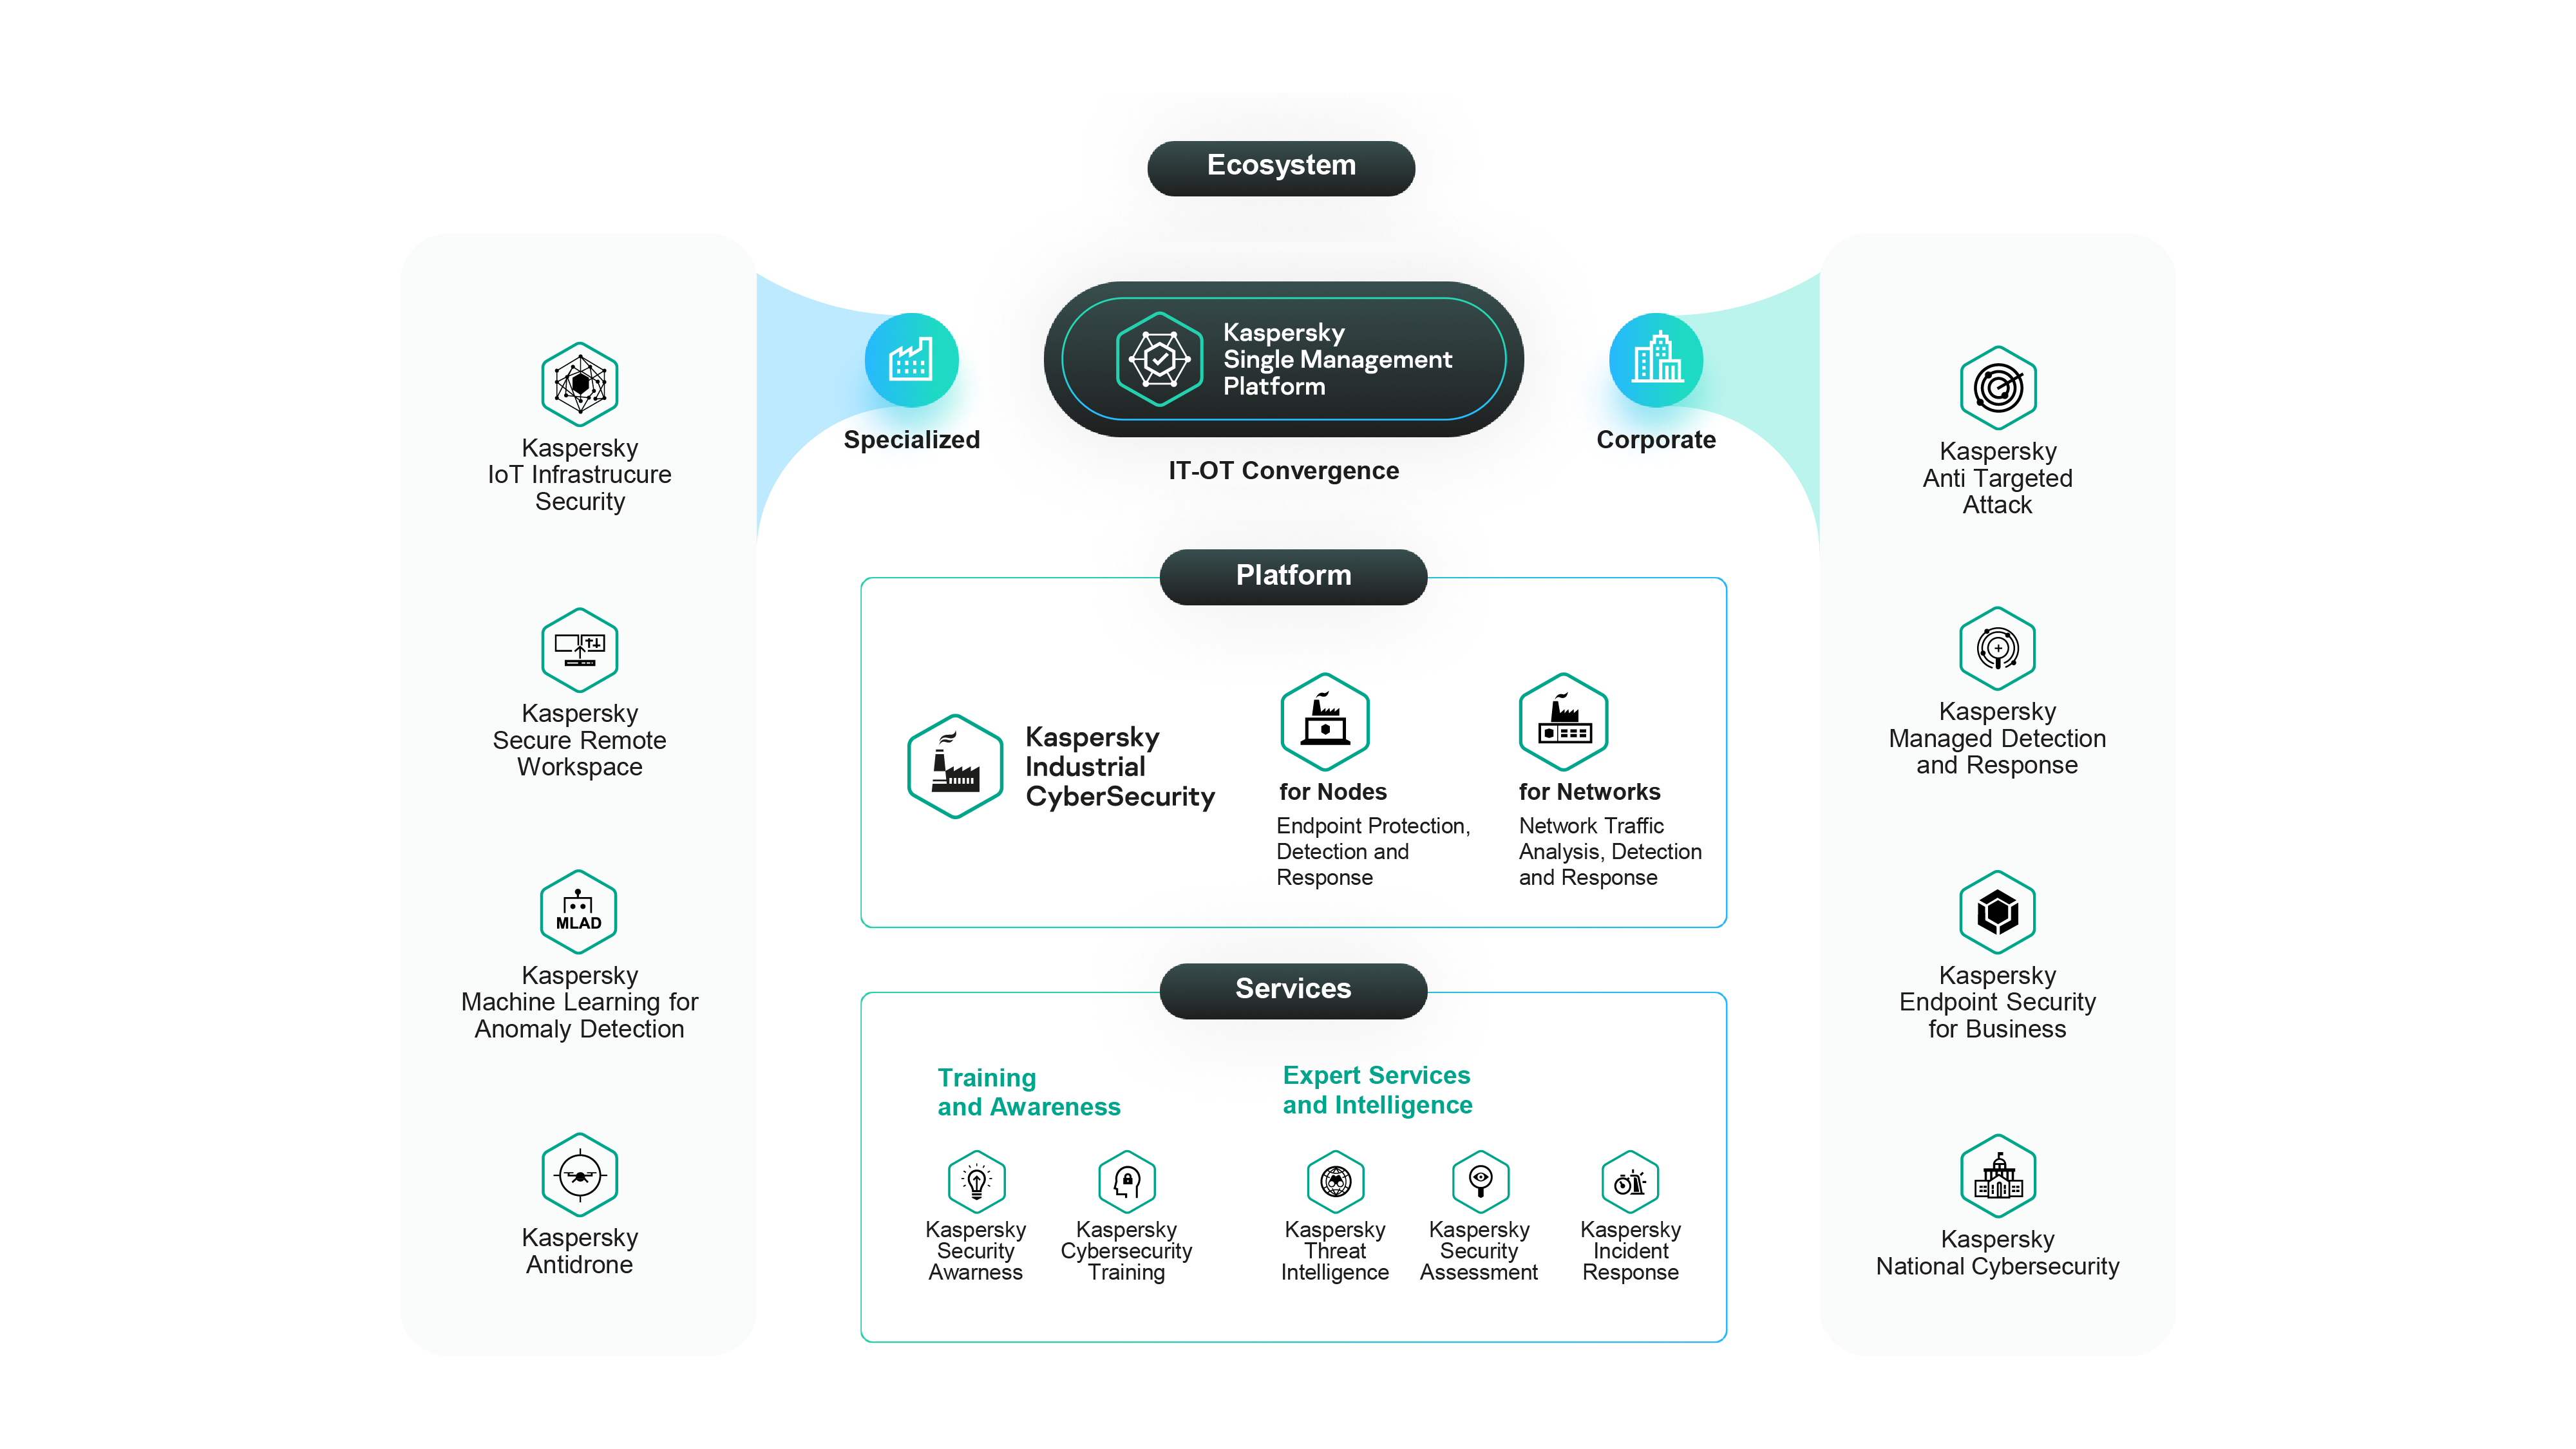
\includegraphics[width=0.95\columnwidth]{images/KICS.png}
   \caption{\textsc{KICS} schema}
   \label{fig:KICS}
\end{figure}
\colfill

\end{paracol}
\section{Ataque sobre la infraestructura industrial y defensa}

El ataque que se muestra en el video comprende tres fases, también se analizan las posibles implementaciones de cada una de ellas:
\begin{enumerate}
   \item \textbf{Breach} - \textit{Obtener acceso a un componente}
   \begin{itemize}
      \item Instalar un malware a traves de un documiento \texttt{.pdf} en un \textsc{usb}, que cuando se abre, se conecta al atacante, que obtiene acceso la computadora infectada, que puede utilizar como fuente para futuros ataques en la red.
      \item \textit{\ul{Defensa}} - \textsc{KICS} for Networks detecta una comunicación no autorizada entre la computadora infectada y una dirección IP externa y un payload potencialmente peligroso, y envía una alerta a \textit{Kaspersky Security Center}.
      \note{Si puede bloquear el ataque aquí, pero en el video se supone que no lo haces para mostrar el comportamiento defensivo en las fases siguientes}
      \begin{figure}[htbp]
         \centering
         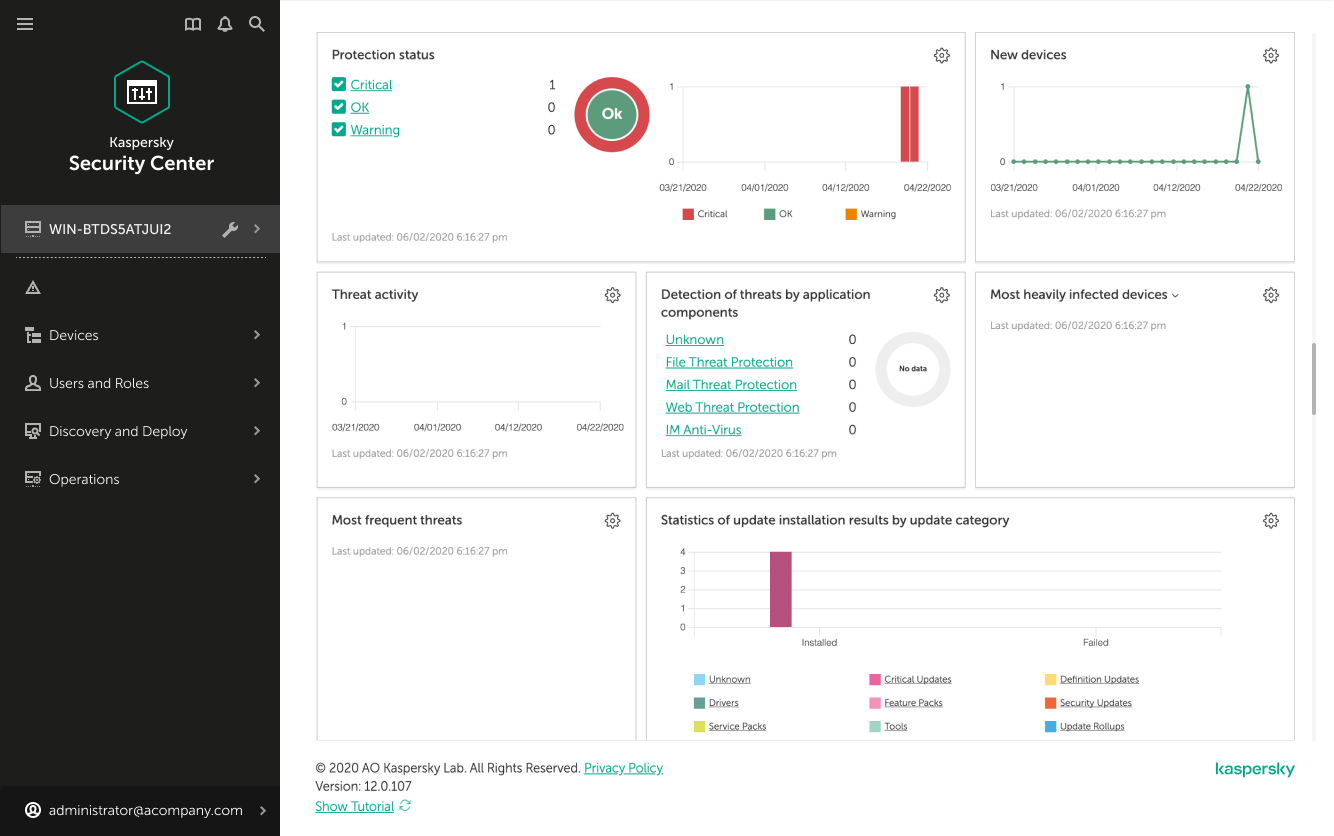
\includegraphics{images/KasperskySC.png}
         \caption{Kaspersky Security Center}
         \label{fig:KasperskySC}
      \end{figure}
   \end{itemize}
   \item \textbf{Discovery} - \textit{Obtener información y datos sobre el sistema}
   \begin{itemize}
      \item A través del componente infectado, el atacante puede \textbf{escanear} la red y obtener información sobre los dispositivos ciber y ciberfísicos conectados, lo que le permite establecer las vulnerabilidades actuales y planificar futuros ataques explotándolas.
      A menudo las comunicaciones entre dispositivos ciberfísicos y ciber carecen de \textbf{encriptación}, potencialmente exponiendo datos y credenciales sensibles.\\
      Si no hay suficiente segmentación de red, o si falta apropiada configuración de los Firewalls, este proceso puede ser aún más facilitado.
      \item \textit{\ul{Defensa}} - \textsc{KICS} for Networks detecta un escaneo de red no autorizado y envía una alerta a Kaspersky Security Center. Imagino que \textsc{KICS} también puede detectar cualquier movimiento lateral del atacante.
   \end{itemize}
   \item \textbf{Technlogical Attack} - \textit{Ataque a la infraestructura}
   \begin{itemize}
      \item Si no se bloquea el ataque en la fase anterior, el atacante puede enviar \textbf{comandos no autorizados} (\textit{command injection}) a los dispositivos ciberfísicos.\\
      El ejemplo que se hace en el video es de utilizar una vulnerabilidad ---conocida--- del firmware del componente de protección del transformador para enviar un comando inapropiado para updatear el firmware de modo que el dispositivo deje de cumplir su función de protección.

      \note{Vulnerabilidades típicas de sistemas CPS incluyen:\ns
      \begin{itemize}
      	\item Permissions, Privileges and Access Control
	      \item Improper Authentication
	      \item Insufficient Verification of Data Authenticity
      \end{itemize}
      Parece claro como estas pueden facilitar un ataque como el que se muestra en el video.}
      \item En este punto, el atacante puede causar daños físicos como cortocircuitos y similares
      \item \textit{\ul{Defensa}} - \textsc{KICS} for Networks detecta un comando no autorizado y envía una alerta a Kaspersky Security Center.\\
      Aunque no se detenga el ataque, podemos utilizar la información recopilada para mitigar futuros ataques.
   \end{itemize}
\end{enumerate}

% \framedt{
%    GOOSE spoofing
% }{
%    GOOSE spoofing es un ataque que consiste en enviar mensajes GOOSE (Generic Object Oriented Substation Event) falsos a los dispositivos de la subestación, lo que puede provocar fallos en el sistema.
% }

\subsection{Conclusiones sobre \textsc{KICS}}
El vídeo no discute en profundidad la defensa de \textsc{KICS}, pero me parece que el punto de fuerza de \textsc{KICS} sea que puede operar a diversos \textbf{niveles}, y que instancias de \textsc{KICS} pueden \textbf{comunicarse} entre sí para compartir información sobre ataques y vulnerabilidades.
Esto permite de hacer un análisis de lo que está ocurriendo más \textbf{completa} y \textbf{amplia}, que es el punto fundamental de la Ciberconciencia Situacional.

Sin embargo, el problema fundamental en sistemas ICS es que luego de detectar un ataque, hay que decidir como responder a él, porque \ul{no se puede hacer nada que pueda interrumpir o alterar el funcionamiento del sístema}, las prioridades son la continuidad del servicio, y la seguridad del personal y de la infraestructura.\\
Esto es un problema que no se discute en el video y cuya gestión puede depender mucho del sistema concreto en cuestión.
\chapter{Estrategias de Testing}
\label{chap:estrategias-de-testing}

El proceso de testng dentro de un proyecto de software es una actvidad que tene como objetivo \ul{verificar} y \ul{validar} que el software cumple con los requisitos especificados.

El proceso de testing conlleva:
\begin{itemize}
	\item planificación,
	\item diseño,
	\item ejecución de pruebas y
	\item evaluación
\end{itemize}
La gestión de calidad debe garan2zar que el proceso de
testing se lleve a cabo de manera eficiente y eficaz.

\section{Tipos de Testing}
\begin{itemize}
	\item Testeo \textbf{unitario}\\
   Testeo de unidades de software individuales
	\item Testeo de \textbf{integración}\\
   Testeo de los interfaces de y la interacción entre las unidades previamente testeadas
	\item Testeo de \textbf{sistema}\\
   Testeo del sistema entero
	\item Testeo de \textbf{aceptación}\\
   Testeo del sistema y los criterios de aceptación previamente establecidos con el cliente
\end{itemize}

\subsection{Testeo Unitario}
Las \textbf{unidades} son Clases/Métodos (en OO), Procedimientos, Módulos o Componentes. Como se definen las unidades depende del diseño, de la criticidad del software (más crítico implica unidades más pequeñas), de la empresa (estrategia), o del tiempo disponible.


Una \textbf{prueba unitaria} (\texttt{unit test}) es una pieza de código escrita por un desarrollador que pone a prueba un pequeño y específico trozo de código.
Es una manera relativamente barata para mejorar la calidad del código producido, pero \textit{NO} es para usuarios, gerentes, jefes de proyectos: està hech para los programadores.
El programador examina o ejecuta una pequeña
parte de su código, para testear:
\ul{la funcionalidad que él o ella piensa que tiene que tener}

\begin{figure}[htbp]
   \centering
   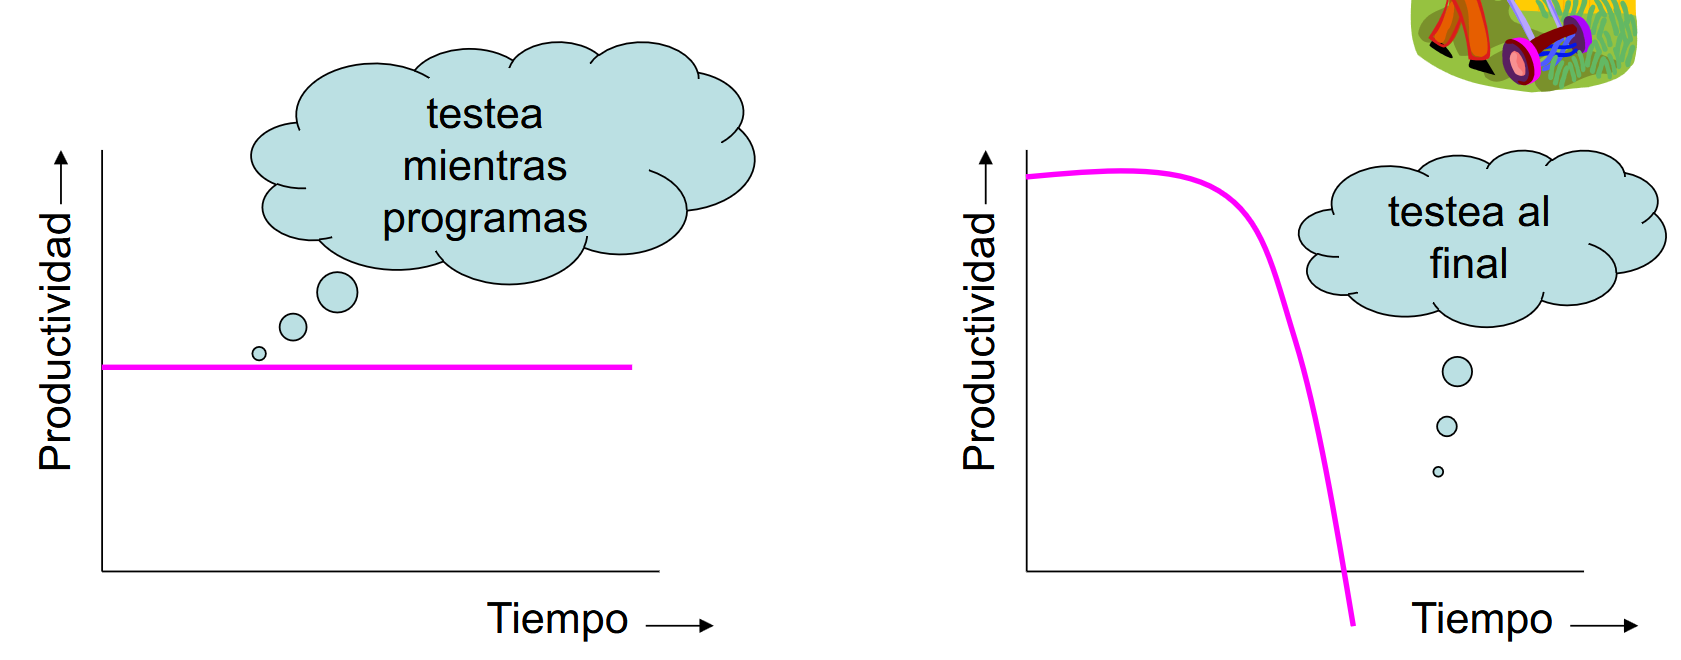
\includegraphics{images/03/unitPostpone.png}
   \caption{Posponer el testeo unitario cuesta mucho tiempo}
   \label{fig:03/unitPostpone}
\end{figure}

\coolquote{
   No es mi trabajo hacer testeo, tenemos un departamento de calidad
}{Bad programmer}

Entonces ¿cuál es el trabajo de un programador? El trabajo de cada programador es \ul{producir código que
funciona y que no contenga ``muchos'' errores}

\subsubsection{JUnit}

\begin{paracol}{2}
	
	\colfill
	JUnit es un framework de testing para Java. JUnit es una herramienta que ayuda a los programadores a escribir pruebas unitarias en Java. JUnit ha sido importante en el desarrollo de la metodología de programación extrema (XP).
	\lstinline|@Test| son los métodos de prueba.
	\begin{itemize}
		\item \lstinline|@BeforeEach| se invoca antes de la ejecución de cada test
		\item \lstinline|@AfterEach| se invoca después de la ejecución de cada test
		\item \lstinline|@BeforeAll| se invoca antes de la ejecución de todos los tests
		\item \lstinline|@AfterAll| se invoca después de la ejecución de todos los tests
	\end{itemize}
	
	\colfill
	\switchcolumn

	\begin{lstlisting}
public class TestDB {
	static private Connection dbConn;
	static private Account acc;
	@BeforeAll
	public static void setUpBeforeAll(){
		dbConn = new Connection("Oracle",15,fred, "f");
		dbConn.connect();
	}
	@AfterAll
	public static void tearDownAfterAll(){
		dbConn.disconnect();
		dbConn = null;
		}
	@BeforeEach
	protected void setUp(){
		acc = new Account();
		}
	@AfterEach
	protected void tearDown(){
		acc = null;
	}
	
	public void testAccountAccess(){
	.../Uses dbConn and acc
	}
	public void testEmployeeAccess(){
		.../Uses dbConn and acc
		}
\end{lstlisting}			
\end{paracol}

\begin{paracol}{2}
	
	\colfill
	En el ejemplo anterior, se muestra un test de una clase \texttt{Account} que tiene una conexión a una base de datos. Se puede ver que se crea una conexión a la base de datos en el método \texttt{setUpBeforeAll} y se cierra en el método \texttt{tearDownAfterAll}. Además, se crea una instancia de la clase \texttt{Account} en el método \texttt{setUp} y se destruye en el método \texttt{tearDown}.
	\colfill
	
	\switchcolumn
	Los metodos son ejecutados en el siguiente orden:
	\ns
	\begin{itemize}
		\item \lstinline|setUpBeforeAll|
		\item \lstinline|setUp|
		\item \lstinline|testAccountAccess|
		\item \lstinline|tearDown|
		\item \lstinline|setUp|
		\item \lstinline|testEmployeeAccess|
		\item \lstinline|tearDown|
		\item \lstinline|tearDownAfterAll|
	\end{itemize}
\end{paracol}

% TODO ejemplo factorial

\subsection{Testeo de Integración}

\begin{definition}
	[Testeo de Integración]
	El testing de las interfaces y la
	interacción entre las unidades previamente testeadas
	mientras que se ensambla el sistema entero
\end{definition}

\begin{itemize}
	\item ¿Qué componentes son el foco del testeo de integración?
	\item ¿En qué orden vamos a testear las interfaces?
	\item ¿Qué técnicas utilizamos para testear las interfaces?
\end{itemize}

Hay tres estrategias:
\begin{enumerate}
	\item \textbf{Big Bang} (todos los componentes a la vez)
	\item \textbf{Bottom-up} (de abajo hacia arriba)
	\item \textbf{Top-down} (de arriba hacia abajo)
\end{enumerate}

\begin{figure}[htbp]
	\centering
	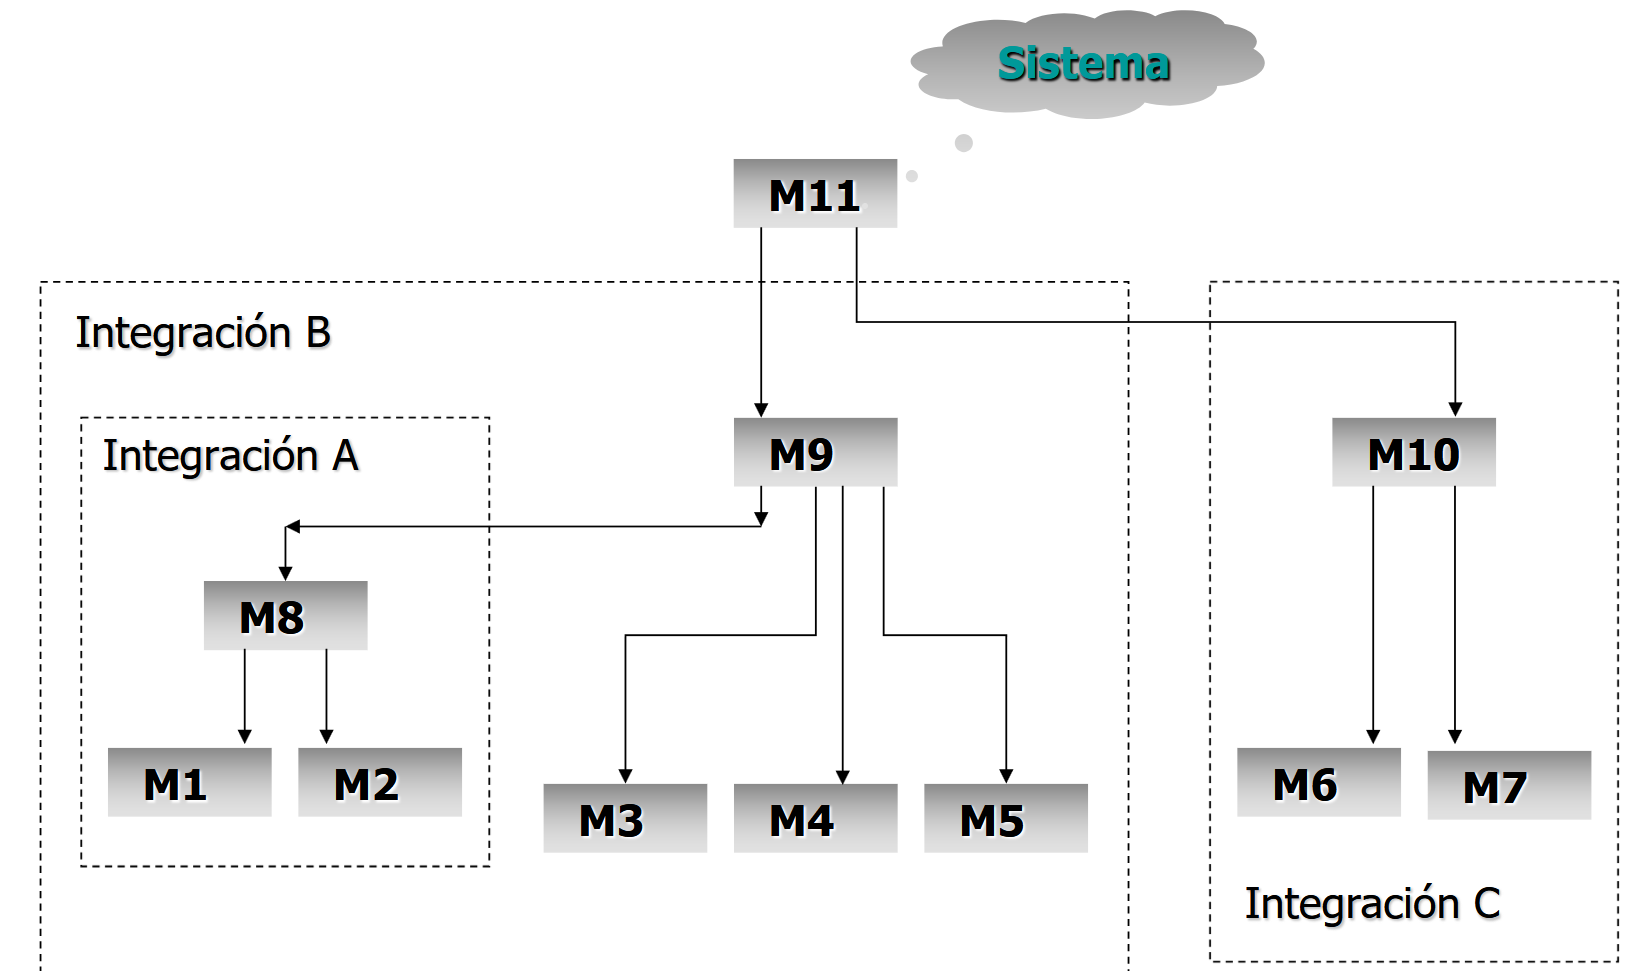
\includegraphics{images/03/bottomup.png}
	\caption{Arbol de dependencia y Bottom-up testing}
	\label{fig:03/bottomup}
\end{figure}

Para hacer el testing \textit{bottom-up} necesitamos \textbf{drivers}.
Un driver es un programa que invoca un componente bajo testeo, por ejemplo, para simular un componente de un nivel superior cuyo código todavía no está disponible (está todavía en desarrollo).

\begin{figure}[htbp]
	\centering
	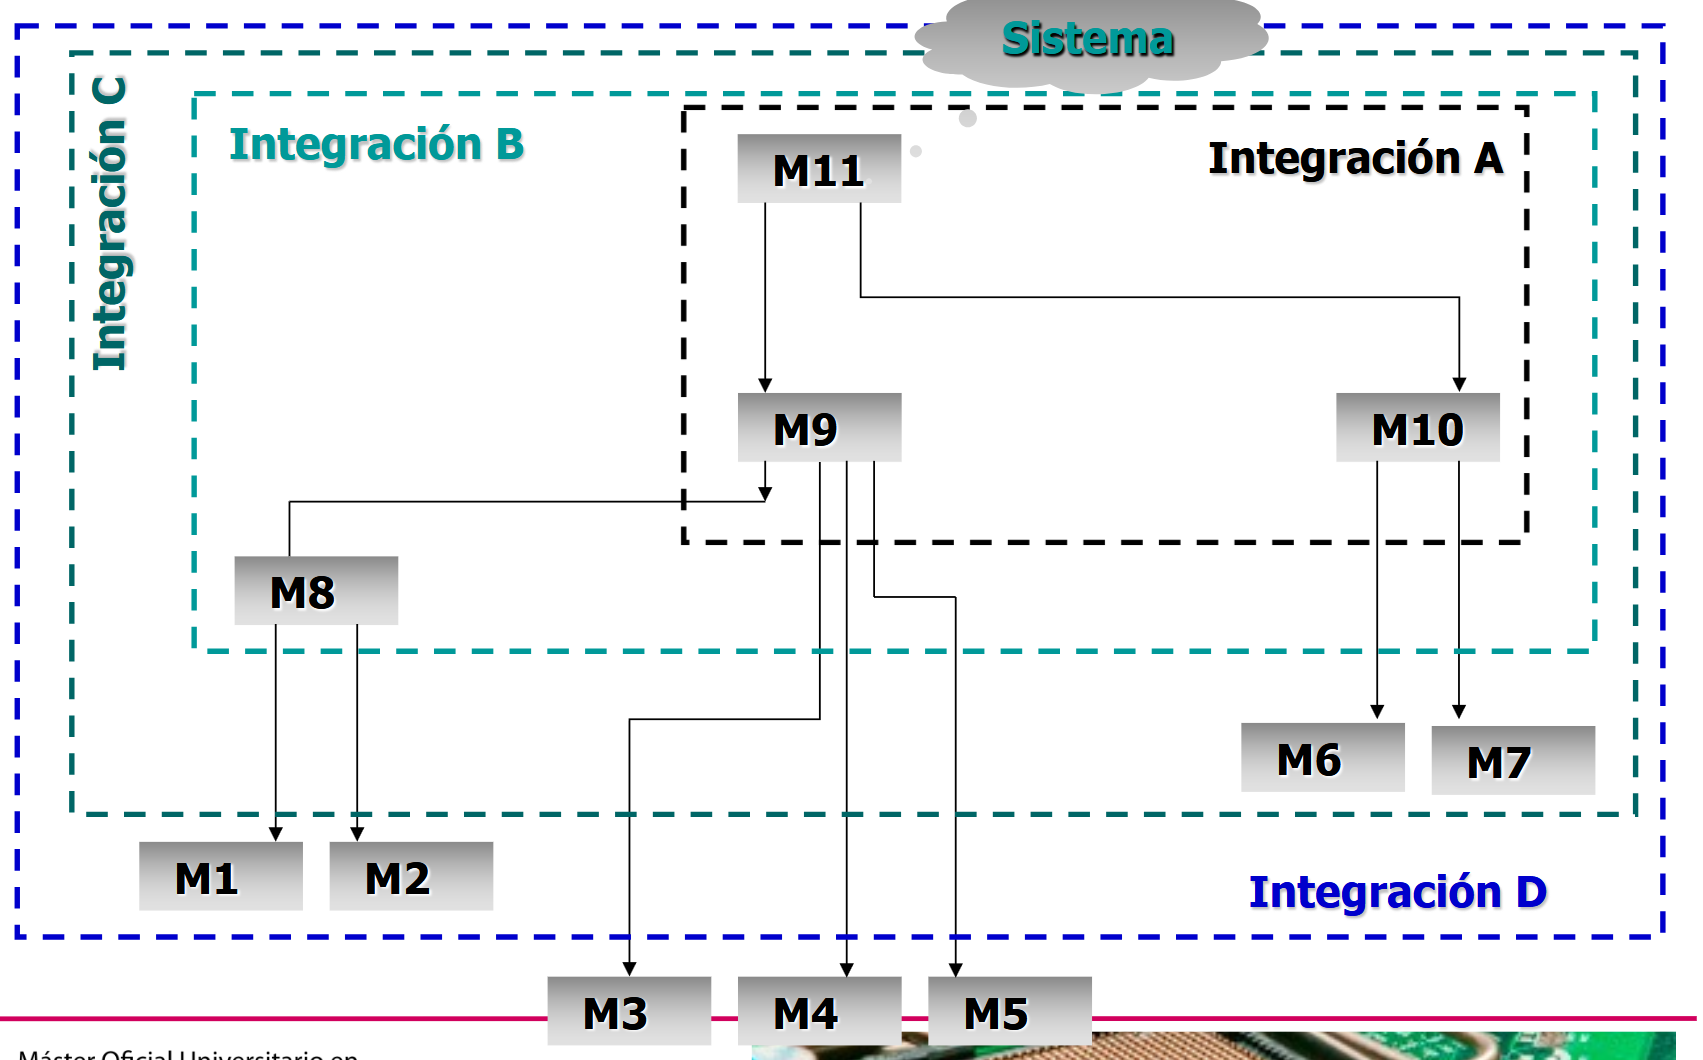
\includegraphics{images/03/topdown.png}
	\caption{Top-down testing}
	\label{fig:03/topdown}
\end{figure}

Para hacer el testeo de integración de manera \textit{top-down}, se
necesita dobles, que simulan componentes de un nivel inferior (``Stub'', ``dummy'', ``fake'', ``mock'').
\ns

El \textit{Big Bang} testing se utiliza solo para sistemas pequeños, ya que es muy difícil de manejar en sistemas grandes.


\subsubsection{Mockito}
Mockito es un framework de testing para Java que permite crear objetos simulados (mocks) de clases y interfaces. Mockito se utiliza para simular objetos que son necesarios para realizar pruebas unitarias. Se puede integrar con JUnit para realizar pruebas unitarias en Java. 
En las slides se muestran ejemplos de cómo utilizar Mockito.

Mockito es muy comodo para implementar el testeo de integración de manera \textit{top-down}.
% TODO Parte 2 y 3	

\section{Testeo de Sistema}
Se verifica que se cumple los requisitos especificados, es decir, que el sistema realiza correctamente todas las funcionesque se han detallado en las especificaciones dadas por el usuario del sistema.

Es necesario automatizar las prubas, y por esto se utilizan herramientas como \textit{Selenium}, que permite automatizar pruebas en navegadores web: en este caso, hablamos de pruebas de \textbf{funcionalidad}.

Para testar el \textbf{rendimiento} (tiempo de respuesta, carga, memoria.) se utilizan herramientas como \textit{JMeter} o \textit{NeoLoader}.

Otros aspectos importantes que el testeo debe cubrir son \textbf{Seguridad} y \textbf{Usabilidad}.

\section{Testeo de aceptación}
Esto testeo es dirigido a los criterios de aceptación
previamente establecidos con el cliente. Se puede hacer de manera manual o automatizada.

\subsection{Regresión}
Testeo que se necesita hacer después de cambios en el
software para asegurar que no se ha introducido defectos.

\ul{El testeo de \textbf{regresión} se tiene que automatizar} por el simple hecho de que el testeo de regresión manual \textit{NO SE HACE}.

\section{Gestión de Defectos, métricas y mas}

{El proceso de clasificación de defectos incluye tres fases:\ns
\begin{enumerate}
	\item Detección de defectos
	\item Investigación de defectos
	\item Resolución de defectos
\end{enumerate}}

\note{
\begin{itemize}
	\item \textbf{Actividad} (que estábamos haciendo cuando encontramos el fallo)
	\item \textbf{Fase del proyecto} (en que estábamos cuando encontramos el fallo)
	\item \textbf{Repetitividad} (¿se puede repetir el error?)
	\item \textbf{Síntoma} (fallo del sistema, mensaje de error, entrada no aceptado, resultado
incorrecto, etc.)
	\item \textbf{Causa} (nuestro producto, componente externo, usuario, etc.)
	\item \textbf{Origen} (especificación de requisitos, diseño, programación, etc.)
	\item \textbf{Impacto} (misión: crítico, medio, …; en la planificación; para el cliente, etc.)
\end{itemize}
}

\subsection{Métricas}


 Las métricas son observaciones cuantitativas para:
\begin{itemize}
	\item Informar sobre el \textbf{progreso del proyecto} de testeo
\note{\begin{itemize}
	\item ¿Qué tareas han terminado en tiempo?
	\item ¿Qué tareas han terminado antes?
	\item ¿Qué tareas han tenido retraso?
	\item ¿Cómo vamos siguiendo la planificación?
	\item Si no vamos bien, ¿cuáles son las razones?
	\item ¿Qué productividad ha tenido persona/equipo X?
\end{itemize}}
	\item Informar sobre la \textbf{calidad del software}
	\note{\begin{itemize}
		\item ¿Podemos parar el testeo?
	\item ¿Podemos entregar producto?
	\item ¿Hemos resueltos todos los defectos?
	\item ¿Cómo estamos gesHonando los defectos?
	\item ¿Cuántos defectos hemos encontrado por: subsistema,
	origen, causa, severidad, etc\dots?
	\end{itemize}}
	\item Informar sobre la \textbf{calidad del testeo}
	\note{\begin{itemize}
		\item ¿Estamos haciendo los tests necesarios?
		\item ¿Están siendo efectivos los tests?
		\item ¿Estamos utilizando los casos de prueba adecuados?
		\item ¿Necesitamos tener en cuenta diferentes casos de prueba?
	\end{itemize}}
\end{itemize}

La cobertura del testeo es una métrica importante para evaluar la calidad del testeo. La cobertura del testeo es la medida de la cantidad de código que ha sido ejecutado por los tests, especialmente en lo que se refiere a instrucciones, decisiones y condiciones (múltiples).\\
Pero puede referirse también a la cobertura de los requisitos, de los casos de uso, de los casos de prueba, etc.

\begin{lstlisting}[caption={Con 1 test donde \lstinline|x==y| se cubre todo el codigo, pero no todas las decisiones. En efecto, el defecto ocurre cuando \lstinline|x!=y|}]
	int foo_3 ( ) {
		int* p = NULL;
		int x;
		if (x==y) {
			p = &x;
		}
		*p = 123;
	}
\end{lstlisting}

\subsection{Mutación}

La mutación es una técnica de testing que consiste en introducir errores en el código fuente para ver si los tests son capaces de detectarlos. Se puede utilizar para evaluar la calidad de los tests.

\subsection{Organización del testing}
Se puede dedicar un equipo de testo integrado, con un jefe, o se puede haber que desarrolladores y testeadores son las mismas personas y no hay testeadores a tiempo completo.
La ventaja de tener un equipo de testeo es que se puede tener una visión más objetiva del software, ya que los testeadores no han desarrollado el software; al contrario, si los desarrolladores hacen el testeo, no tienen que comunicar con los testeadores, y conocen el software.

Otra tecnica de organización es \textit{Outsourcing}, que consiste en contratar una empresa externa para hacer el testeo. La ventaja es que se puede tener una visión más objetiva del software, y se puede tener acceso a expertos en testeo. La desventaja es que se puede tener problemas de comunicación, y que se puede tener problemas de confidencialidad.


\chapter{Cluster analysis}


Finding groups of objects such that the objects in a group
will be similar (or related) to one another and different
from (or unrelated to) the objects in other groups.

The aim of clustering is to ease data \textbf{understanding} and \textbf{summarization}, i.e. reduce the size of data sets.

\note{
	The following are \textit{NOT} cluster analysis:
	\begin{itemize}
		\item Simple segmentation
		\begin{itemize}
			\item Dividing students into different registration groups
		\end{itemize}
		alphabetically, by last name
		\item Results of a query
		      \begin{itemize}
			      \item Groupings are a result of an external specification
			      \item Clustering is a grouping of objects based on the data
		      \end{itemize}
		\item Supervised classification
		      \begin{itemize}
			      \item Have class label information
		      \end{itemize}
		\item Association Analysis
		      \begin{itemize}
			      \item Local vs. global connections
		      \end{itemize}
	\end{itemize}

	These ain't clustering essentially because there is no \textbf{similarity} measure involved, which instead is the core of clustering.
}

\begin{figure}[htbp]
   \centering
   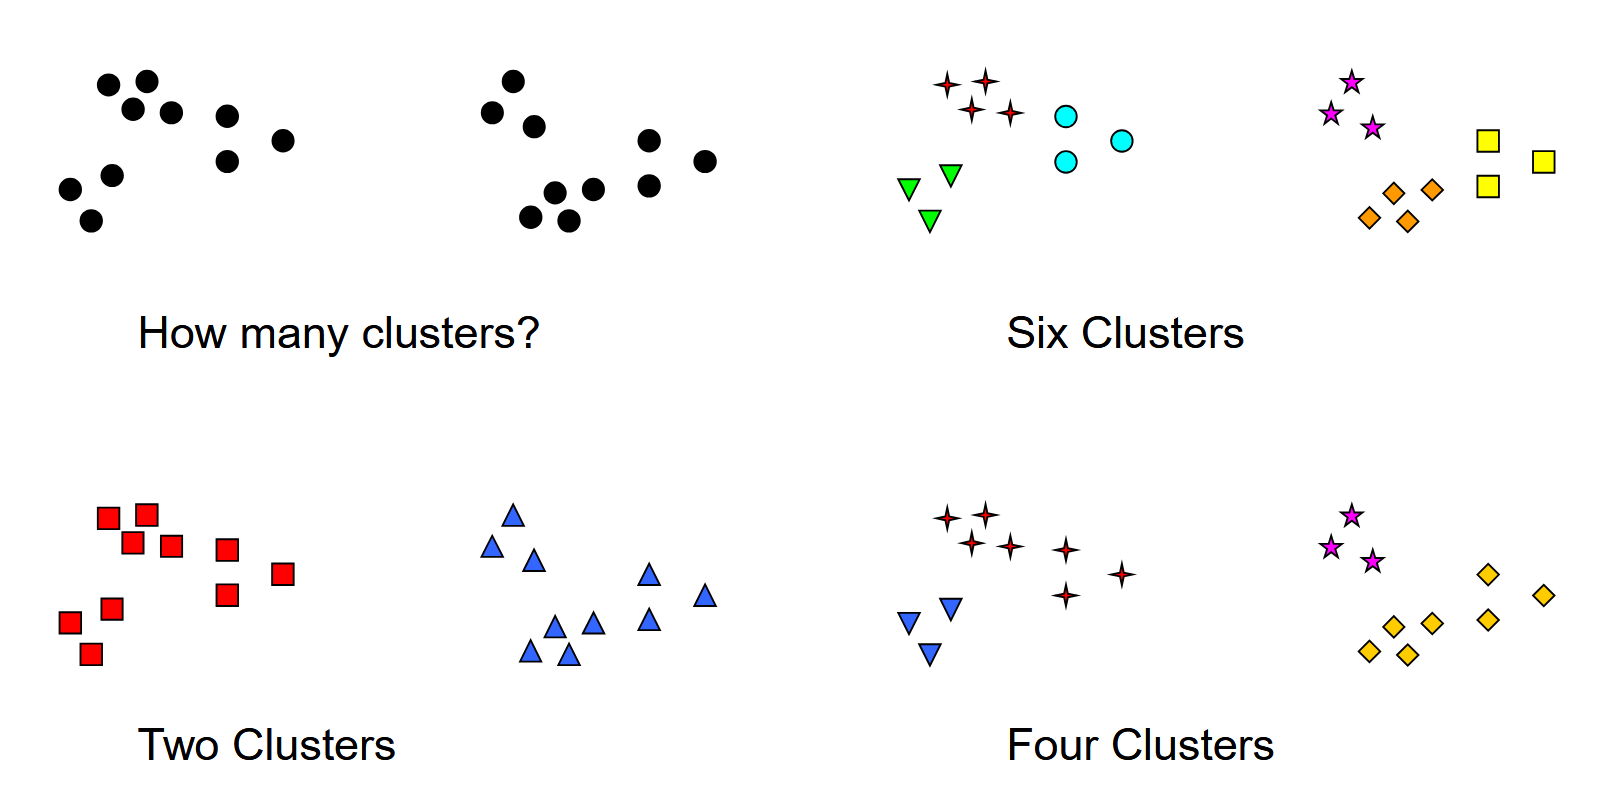
\includegraphics{images/04/clustering.png}
   \caption{``Cluster'' may be an amibguous term. How to define a cluster? How big is a cluster? How many clusters are there?}
   \label{fig:04/clustering}
\end{figure}

\section{Definitions}
A \textbf{clustering} is a set of clusters. There is an important distinction between hierarchical and
partitional sets of clusters.
\begin{itemize}
	\item \textit{Partitional} Clustering\\
	A division of data objects into non-overlapping subsets
	(clusters) such that each data object is in exactly one subset.
	\item \textit{Hierarchical} Clustering\\
	A set of nested clusters organized as a hierarchical tree.
\end{itemize}

\begin{figure}[htbp]
	\centering
	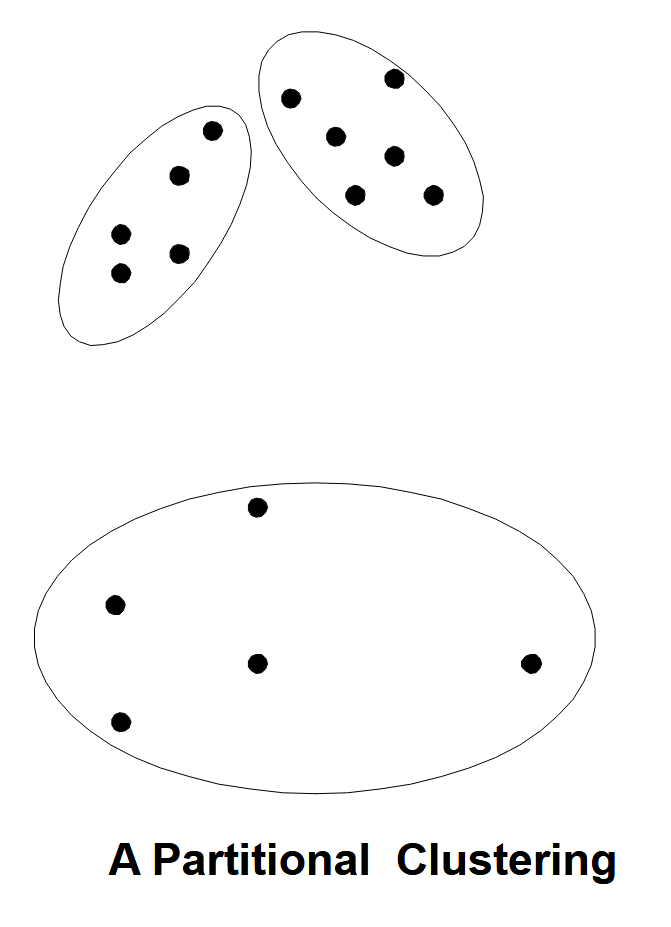
\includegraphics[width=0.33\columnwidth]{images/04/partitional.png}
	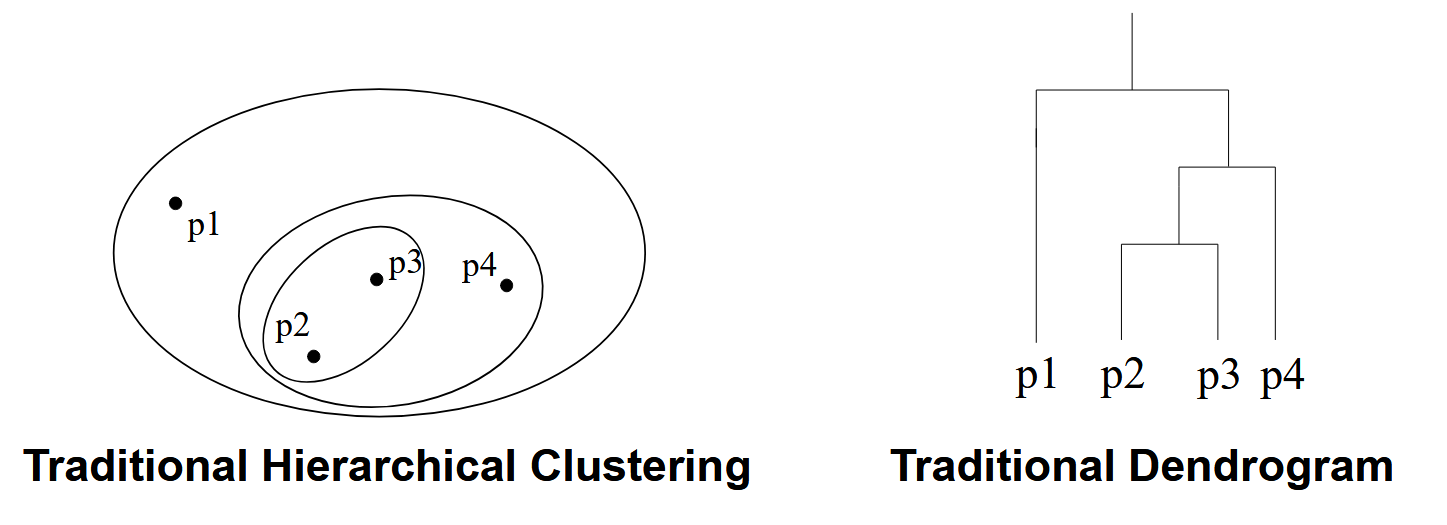
\includegraphics[width=0.66\columnwidth]{images/04/hierarchical.png}
	\caption{Partitional vs Hierarchical clustering}
	\label{fig:04/partitional_hierarchical}
\end{figure}


There are other distinctions among clusterings:
\begin{itemize}
	\item Exclusive versus non-exclusive
	      \begin{itemize}
		      \item In non-exclusive clusterings, points may belong to multiple
	      \end{itemize}
	      clusters.
	      \begin{itemize}
		      \item Can represent multiple classes or ‘border’ points
	      \end{itemize}
	\item Fuzzy versus non-fuzzy
	      \begin{itemize}
		      \item In fuzzy clustering, a point belongs to every cluster with some
		            weight between 0 and 1
		      \item Weights must sum to 1
		      \item Probabilistic clustering has similar characteristics
	      \end{itemize}
	\item Partial versus complete
	      \begin{itemize}
		      \item In some cases, we only want to cluster some of the data
	      \end{itemize}
	\item Heterogeneous versus homogeneous
	      \begin{itemize}
		      \item Clusters of widely different sizes, shapes, and densities
	      \end{itemize}
\end{itemize}

\section{Types of Clustering}
% // TODO add pictures
\begin{itemize}
	\item Well-separated clusters
	      A cluster is a set of points such that any point in a cluster is closer (or more similar) to every other point in the cluster than to any point not in the cluster
	\item Center-based clusters
	      \begin{paracol}{2}
		      \begin{figure}[htbp]
			      \centering
			      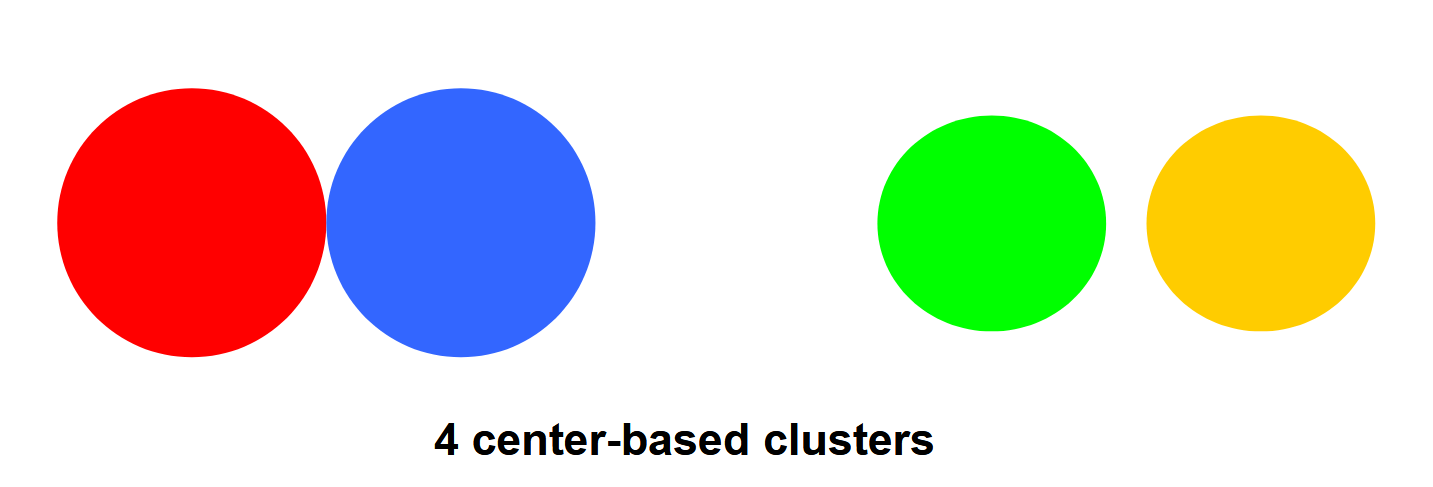
\includegraphics{images/04/centerbased.png}
			      \caption{Center-based clusters}
			      \label{fig:04/centerbased}
		      \end{figure}
		      \switchcolumn

		      \begin{itemize}
			      \item A cluster is a set of objects such that an object in a cluster is
			            closer (more similar) to the “center” of a cluster, than to the
			            center of any other cluster
			      \item The center of a cluster is often a centroid, the average of all
			            the points in the cluster, or a medoid, the most “representative”
			            point of a cluster
		      \end{itemize}
	      \end{paracol}
	\item Contiguous clusters (Nearest neighbor or
	      Transitive)

	      \begin{paracol}{2}
		      \colfill
		      \begin{itemize}
			      \item Each point is closer to at least one point in its cluster than to
			            any point in another cluster.
			      \item Graph based clustering
			      \item This approach can have trouble when noise is present since a
			            small bridge of points can merge two distinct clusters
		      \end{itemize}

		      \colfill
		      \switchcolumn

		      \begin{figure}[htbp]
			      \centering
			      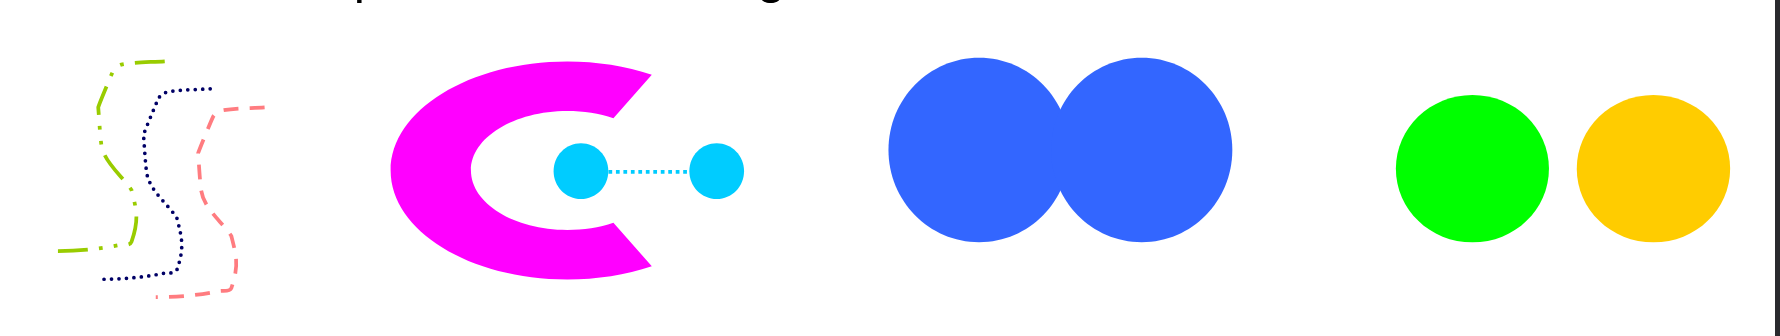
\includegraphics{images/04/contiguitybased.png}
			      \caption{Contiguity-based clusters}
			      \label{fig:04/contiguitybased}
		      \end{figure}

	      \end{paracol}

	\item Density-based clusters
	      \begin{paracol}{2}
		      \colfill
		      \begin{itemize}
			      \item A cluster is a dense region of points, which is separated by
			            low-density regions, from other regions of high density.
			      \item Used when the clusters are irregular or intertwined, and when
			            noise and outliers are present.
			      \item Points which are not classfied as part of any cluster are considered noise. In the figure they may be the gray blackground points.
		      \end{itemize}
		      \colfill
		      \switchcolumn
		      \begin{figure}[htbp]
			      \centering
			      
\includegraphics{images/04/densitybased.png}
			      \caption{Density-based clusters}
			      \label{fig:04/densitybased}
		      \end{figure}
	      \end{paracol}
	\item Property or Conceptual
	\item Described by an Objective Function
	      \begin{itemize}
		      \item Finds clusters that minimize or maximize an objective
		            function.
		      \item Enumerate all possible ways of dividing the points into
		            clusters and evaluate the `goodness' of each potential
		            set of clusters by using the given objective function.
		      \item NP Hard)
		      \item Can have global or local objectives.
		            \begin{itemize}
			            \item Hierarchical clustering algorithms typically have local objectives
			            \item Partitional algorithms typically have global objectives
		            \end{itemize}
	      \end{itemize}
\end{itemize}

\newpage
\section{Similarity}
\begin{itemize}
    \item Similarity
          \begin{itemize}
              \item Numerical measure of how alike two data objects are.
              \item Is higher when objects are more alike.
              \item Often falls in the range [0,1]
          \end{itemize}
    \item Dissimilarity
          \begin{itemize}
              \item Numerical measure of how different are two data objects
              \item Lower when objects are more alike
              \item Minimum dissimilarity is often 0
              \item Upper limit varies
          \end{itemize}
    \item Proximity refers to a similarity or dissimilarity
\end{itemize}

\subsection{Similarity and Dissimilarity for Different Attribute Types}

\begin{table}[htbp]
\centering
\caption{Similarity and dissimilarity for simple attributes}
\begin{tabular}{|p{3cm}|p{6cm}|p{4cm}|}
\hline
\textbf{Attribute Type} & \textbf{Dissimilarity} & \textbf{Similarity} \\
\hline
Nominal & 
$d = \begin{cases}
0 & \text{if } p = q \\
1 & \text{if } p \neq q
\end{cases}$ & 
$s = \begin{cases}
1 & \text{if } p = q \\
0 & \text{if } p \neq q
\end{cases}$ \\
\hline
Ordinal & 
$d = \frac{|p-q|}{n-1}$

(values mapped to integers 0 to $n-1$, where $n$ is the number of values) & 
$s = 1 - \frac{|p-q|}{n-1}$ \\
\hline
Interval or Ratio & 
$d = |p - q|$ & 
$s = -d$, $s = \frac{1}{1+d}$ or

$s = 1 - \frac{d-min\_d}{max\_d-min\_d}$ \\
\hline
\end{tabular}
\label{tab:similarity_attributes}
\end{table}

$p$ and $q$ are the attribute values for two data objects.

\subsection{Euclidean Distance}
The most common way to measure distance between two data objects is the Euclidean distance:

\[
d(\mathbf{x}, \mathbf{y}) = \sqrt{\sum_{k=1}^{n}(x_k - y_k)^2}
\]

where $n$ is the number of dimensions (attributes) and $x_k$ and $y_k$ are, respectively, the $k^{th}$ attributes (components) or data objects $\mathbf{x}$ and $\mathbf{y}$. Standardization is necessary, if scales differ.

\begin{itemize}
    \item Standardization is necessary, if scales differ.
\end{itemize}


\subsubsection{Minkowski Distance}

Minkowski Distance is a generalization of Euclidean Distance. $r$ is a parameter that defines the type of distance, $n$ is the number of dimensions (attributes) and $x_k$ and $y_k$ are, respectively, the $k^{th}$ attributes (components) or data objects $\mathbf{x}$ and $\mathbf{y}$.

\[
d(\mathbf{x}, \mathbf{y}) = \left(\sum_{k=1}^{n} |x_k - y_k|^r\right)^{\frac{1}{r}}
\]

\begin{itemize}
	\item For $r=1$, it is the Manhattan distance (or city block/Hamming distance)
	\item For $r=2$, it is the Euclidean distance
	\item For $r \rightarrow \infty$, it is the supremum distance (or Chebyshev distance)
\end{itemize}

\framedt{Metrics and Similiraties}{
	\begin{enumerate}
		\item $d(x, y) \geq 0$ for all $x$ and $y$ and $d(x, y) = 0$ only if
		      $x = y$. (Positive definiteness)
		\item $d(x, y) = d(y, x)$ for all $x$ and $y$. (Symmetry)
		\item $d(x, z) \leq d(x, y) + d(y, z)$ for all points $x$, $y$, and $z$ (Triangle Inequality).
	\end{enumerate}
	A \textit{distance} $d$ is a \textit{metric} if it satisfies the three conditions above.

	\begin{enumerate}
			\item $s(x, y) = 1$ (or maximum similarity) only if $x = y$.
			\item $s(x, y) = s(y, x)$ for all $x$ and $y$. (Symmetry)
	\end{enumerate}
	These instead are properties of a \textit{similarity} measure.
}

\subsection{Binary Similarity}
Computing similarity among objects described by binary attributes is slightly different from numerical attributes.
\begin{itemize}
	\item Simple Matching Coefficient (SMC)
	      \[
		      SMC = \frac{\texttt{\#matches}}{\texttt{\#attributes}}=\frac{f_{11} + f_{00}}{f_{11} + f_{10} + f_{01} + f_{00}}
	      \]
	\item Jaccard Coefficient
	      \[
		      J = \frac{\texttt{\#}11\texttt{matches}}{\texttt{\#non-zero attribute values}}\frac{f_{11}}{f_{11} + f_{10} + f_{01}}
	      \]
\end{itemize}

\begin{align*}
	p &= 1\ 0\ 0\ 0\ 0\ 0\ 0\ 0\ 0\ 0\\
	q &= 0\ 0\ 0\ 0\ 0\ 0\ 1\ 0\ 0\ 1\\
	f_{01} &= 2 \text{ (\#attributes where } p \text{ was 0 and } q \text{ was 1)}\\
	f_{10} &= 1 \text{ (\#attributes where } p \text{ was 1 and } q \text{ was 0)}\\
	f_{00} &= 7 \text{ (\#attributes where } p \text{ was 0 and } q \text{ was 0)}\\
	f_{11} &= 0 \text{ (\#attributes where } p \text{ was 1 and } q \text{ was 1)}\\
	SMC &= \frac{0 + 7}{10} = 0.7\\
	J &= \frac{0}{0 + 1 + 2} = 0
\end{align*}

\subsection{Cosine Similarity}
Used often in text mining, where each dimension corresponds to a term (word) and the value
of the dimension is the frequency of the term in the document.

If $d_1$ and $d_2$ are two document vectors, then
\[
	\cos( d_1, d_2 ) = (d_1 \cdot d_2) / ||d_1|| ||d_2||
\]
where $\cdot$ indicates vector dot product and $||d||$ is the length of vector $d$.

Example:
\begin{align*}
	d_1 &= 3\ 2\ 0\ 5\ 0\ 0\ 0\ 2\ 0\ 0\\
	d_2 &= 1\ 0\ 0\ 0\ 0\ 0\ 0\ 1\ 0\ 2\\
	d_1 \cdot d_2 &= 3*1 + 2*0 + 0*0 + 5*0 + 0*0 + 0*0 + 0*0 + 2*1 + 0*0 + 0*2 = 5\\
	||d_1|| &= \sqrt{3^2 + 2^2 + 0^2 + 5^2 + 0^2 + 0^2 + 0^2 + 2^2 + 0^2 + 0^2} = \sqrt{42}\\
	||d_2|| &= \sqrt{1^2 + 0^2 + 0^2 + 0^2 + 0^2 + 0^2 + 0^2 + 1^2 + 0^2 + 2^2} = \sqrt{6}\\
	\cos(d_1, d_2) &= \frac{5}{\sqrt{42} * \sqrt{6}} = \frac{5}{\sqrt{252}} \approx 0.315
\end{align*}


\subsection{Correlation}

\begin{paracol}{2}
	
	\begin{figure}[htbp]
		\centering
		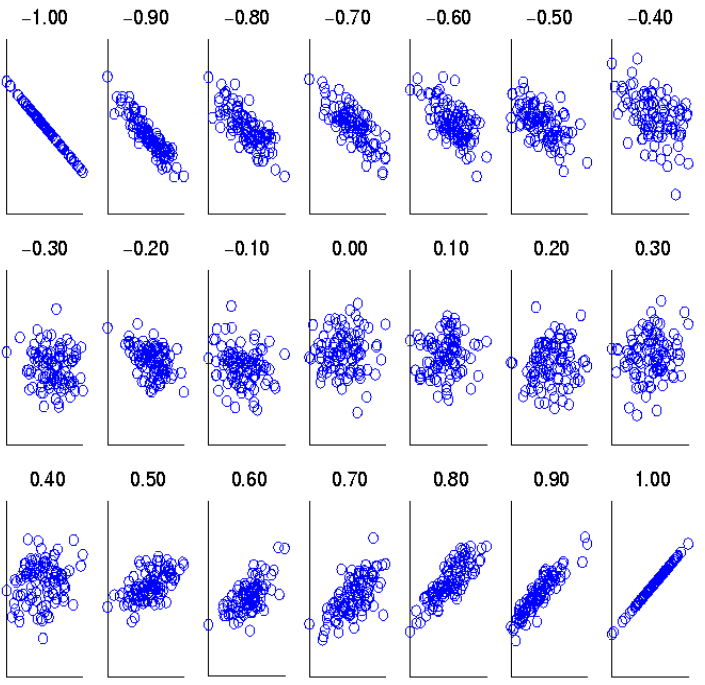
\includegraphics{images/04/correlation.png}
		\caption{Scatter plots showing the similarity from -1 to 1}
		\label{fig:04/correlation}
	\end{figure}
	\switchcolumn
	\colfill
	Correlation measures the linear relationship between objects (binary or continuous).
	To compute correlation, we standardize data objects, $p$ and $q$, and then take their dot product (covariance/standard deviation).
	\colfill
\end{paracol}
	\[
		corr(\mathbf{x},\mathbf{y}) = \frac{covariance(\mathbf{x},\mathbf{y})}{stddev(\mathbf{x})*stddev(\mathbf{y})} = \frac{\sum_{k=1}^{n}(x_k - \bar{x})(y_k - \bar{y})}{\sqrt{\sum_{k=1}^{n}(x_k - \bar{x})^2}\sqrt{\sum_{k=1}^{n}(y_k - \bar{y})^2}}
		\]
		

\subsection{Entropy}
Information relates to possible outcomes of an event such as transmission of a message, flip of a coin, or measurement of a piece of data.
\ul{The amount of information is inversely related to the probability of an event}.
Entropy is the commonly used measure of information content.
For a discrete random variable $X$ with $n$ possible values ${x_1, x_2, ..., x_n}$ each having probability $p_1,p_2,\dots,p_n$, the entropy $H(X)$ is defined as:
\[
H(X) = -\sum_{i=1}^{n} p_i \log_2(p_i)
\]

Entropy is measured in bits and is $0 \leq H(X) \leq \log_2(n)$. Thus, entropy is a measure of how many bits it takes to represent an observation of $X$ on average.

The information one variable provides about another is called mutual information.
The mutual information $I(X;Y)$ of two discrete random variables $X$ and $Y$ is defined as:
\[
I(X,Y) = H(X) + H(Y) - H(X,Y) = \sum_{x \in X} \sum_{y \in Y} p(x,y) \log_2p(x,y)
\]
where $H(X,Y)$ is the joint entropy of $X$ and $Y$, and $p(x,y)$ is the probability that $x$ and $y$ occur together.

\section{K-Means}
\begin{itemize}
	\item \textit{Partitional} clustering approach
	\item The number of clusters $K$, must be specified
	\item Each cluster is associated with a \textbf{centroid} (center point), typically being the mean of the points in the cluster
	\item Each point is assigned to the cluster with the closest centroid. This may measured as Euclidean distance, cosine similarity, correlation, etc.
	\note{Using these measures makes K-Means to converge in the first few iterations.}
	\item Complexity is $O(nKId)$, where $n$ is the number of data points, $K$ is the number of clusters, $I$ is the number of iterations, and $d$ is the number of dimensions (attributes)
	\item The basic algorithm is very simple
\end{itemize}

\begin{algorithm}[H]
\caption{K-Means Clustering Algorithm}
\begin{algorithmic}[1]
\State Select $K$ points as the initial centroids.
\Repeat
\State Form $K$ clusters by assigning all points to the closest centroid.
\State Recompute the centroid of each cluster.
\Until{The centroids don't change}
\end{algorithmic}
\end{algorithm}

\begin{figure}[htbp]
	\centering
	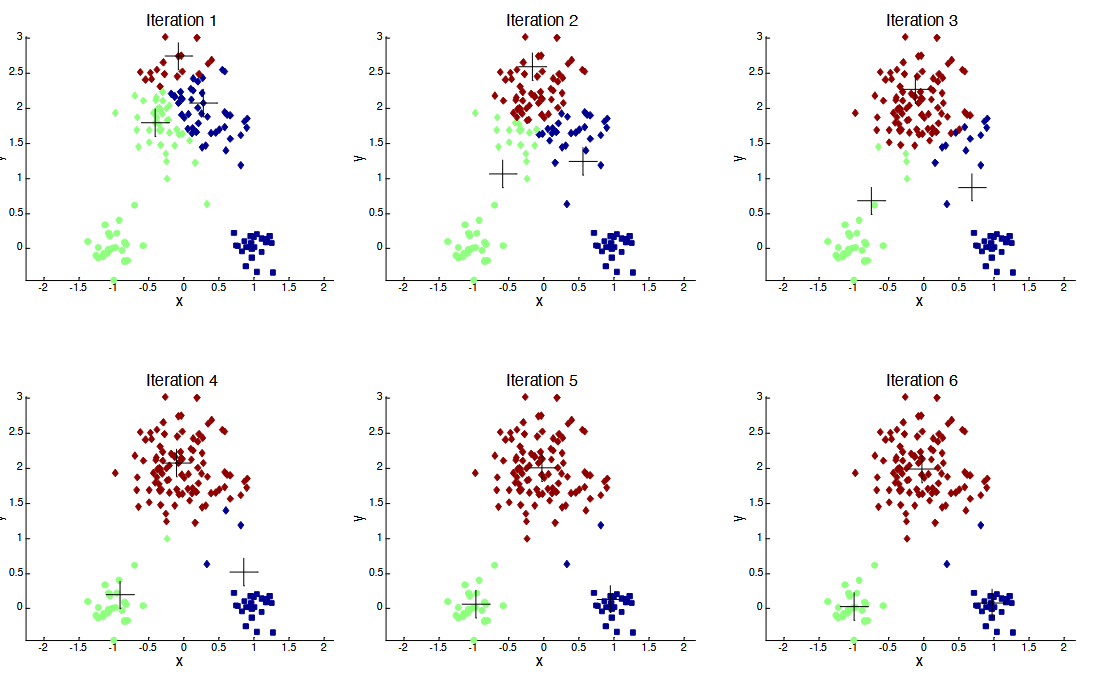
\includegraphics{images/04/kmeans.png}
	\caption{K-Means Clustering Iterations}
	\label{fig:kmeans}
\end{figure}

\subsection{Evaluating K-Means clusters}
The most common measure to evaluate the quality of K-Means clusters is the \textbf{Sum of Squared Errors} (SSE), also known as \textbf{Inertia}. It quantifies how tightly the data points in a cluster are grouped around their centroid. The SSE is calculated as follows:
\[
SSE = \sum_{i=1}^{K} \sum_{x \in C_i} ||x - \mu_i||^2
\]
\note{
	\begin{itemize}
	\item $K$ is the number of clusters,
	\item $C_i$ is the set of points in cluster $i$,
	\item $x$ is a data point in cluster $C_i$,
	\item $\mu_i$ is the centroid of cluster $C_i$,
	\item $||x - \mu_i||^2$ is the squared Euclidean distance between point $x$ and centroid $\mu_i$.
\end{itemize}
}

\subsection{Limitations of K-Means}

\begin{paracol}{2}
	\colfill
	K-means has problems when clusters are of differing
	\begin{itemize}
		\item Clusters have different sizes
		\item Clusters have different densities
		\item Clusters have Non-globular shapes
		\item The data contains \textbf{outliers}.
	\end{itemize}
	\colfill
	\switchcolumn
	\begin{figure}[htbp]
		\centering
		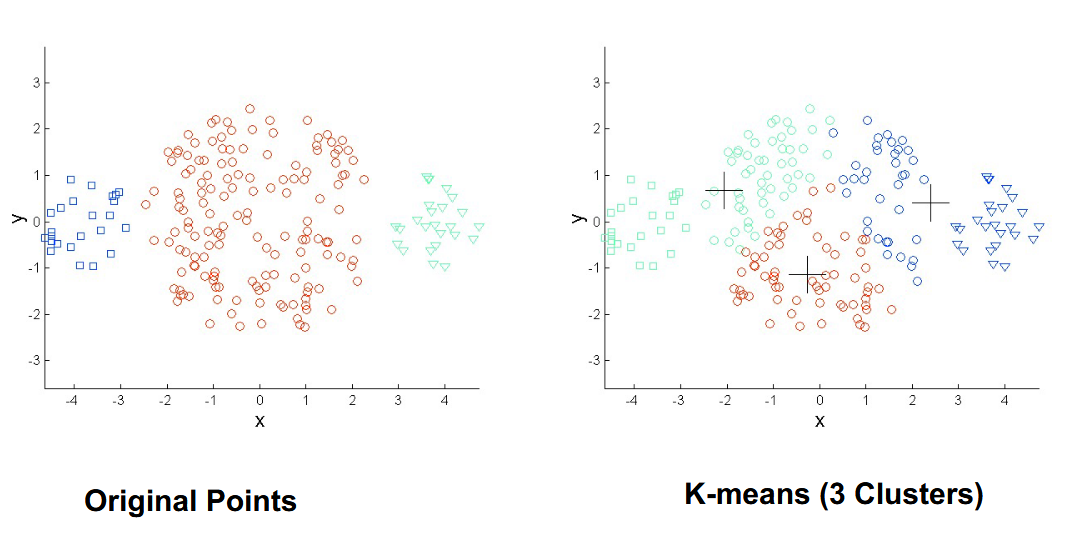
\includegraphics[width=0.9\columnwidth]{images/04/kproblems.png}
		\caption{K-Means with different cluster sizes}
		A solution may be to use more clusters, hence increasing $K$, and then merging them.
		\label{fig:04/kproblems}
	\end{figure}

\end{paracol}

\begin{figure}[htbp]
	\centering
	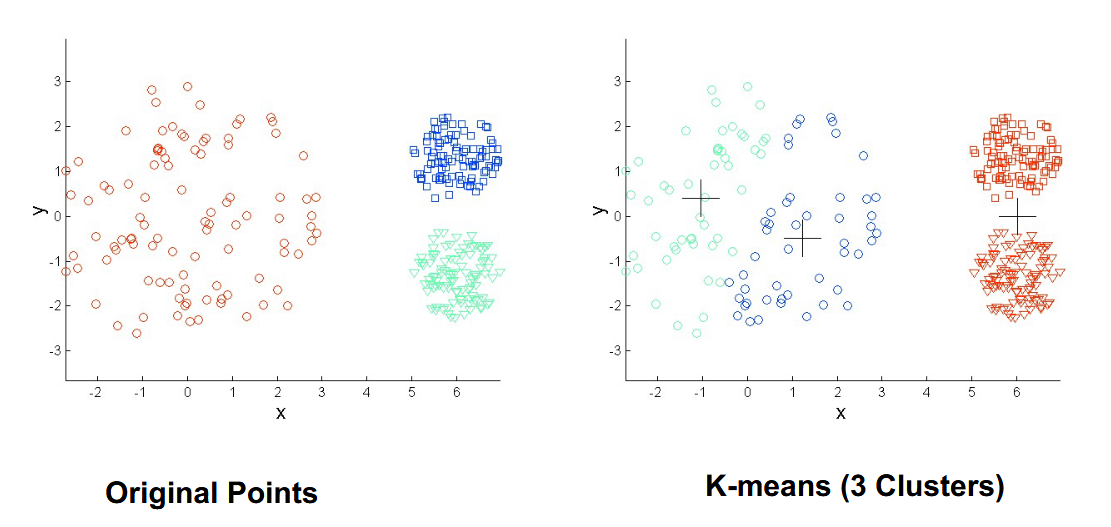
\includegraphics[width=0.48\columnwidth]{images/04/kdensity.png}
	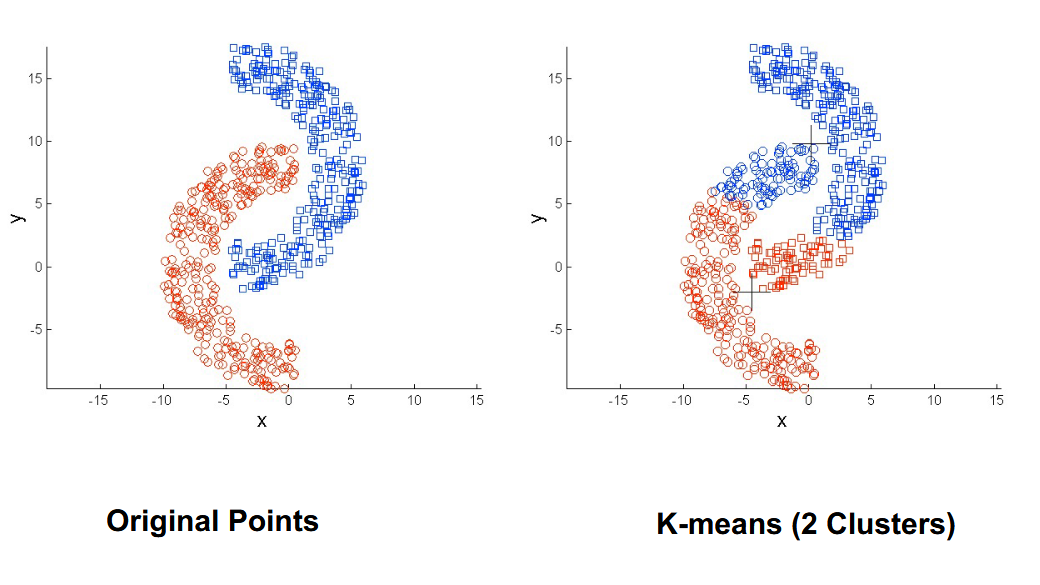
\includegraphics[width=0.48\columnwidth]{images/04/kglobular.png}
	\caption{K-Means with different cluster densities and non-globular shapes}
	\label{fig:04/kdensity}
\end{figure}

\subsubsection{Empty Clusters}

\begin{paracol}{2}
	
	K-Means sometimes produces empty clusters. This happens when no points are assigned to a cluster during the assignment step. This can occur if the initial centroids are poorly chosen or if the data distribution is such that certain centroids end up being too far from any data points.

	 Solutions include the following strategies, which may be iterated until no empty clusters remain:
	\begin{itemize}
		\item Choose a point and assign it to the cluster
		\begin{itemize}
			\item Choose the point that contributes most to SSE
			\item Choose a point from the cluster with the highest SSE
		\end{itemize}
	\end{itemize}

	\switchcolumn

	\begin{figure}[htbp]
		\centering
		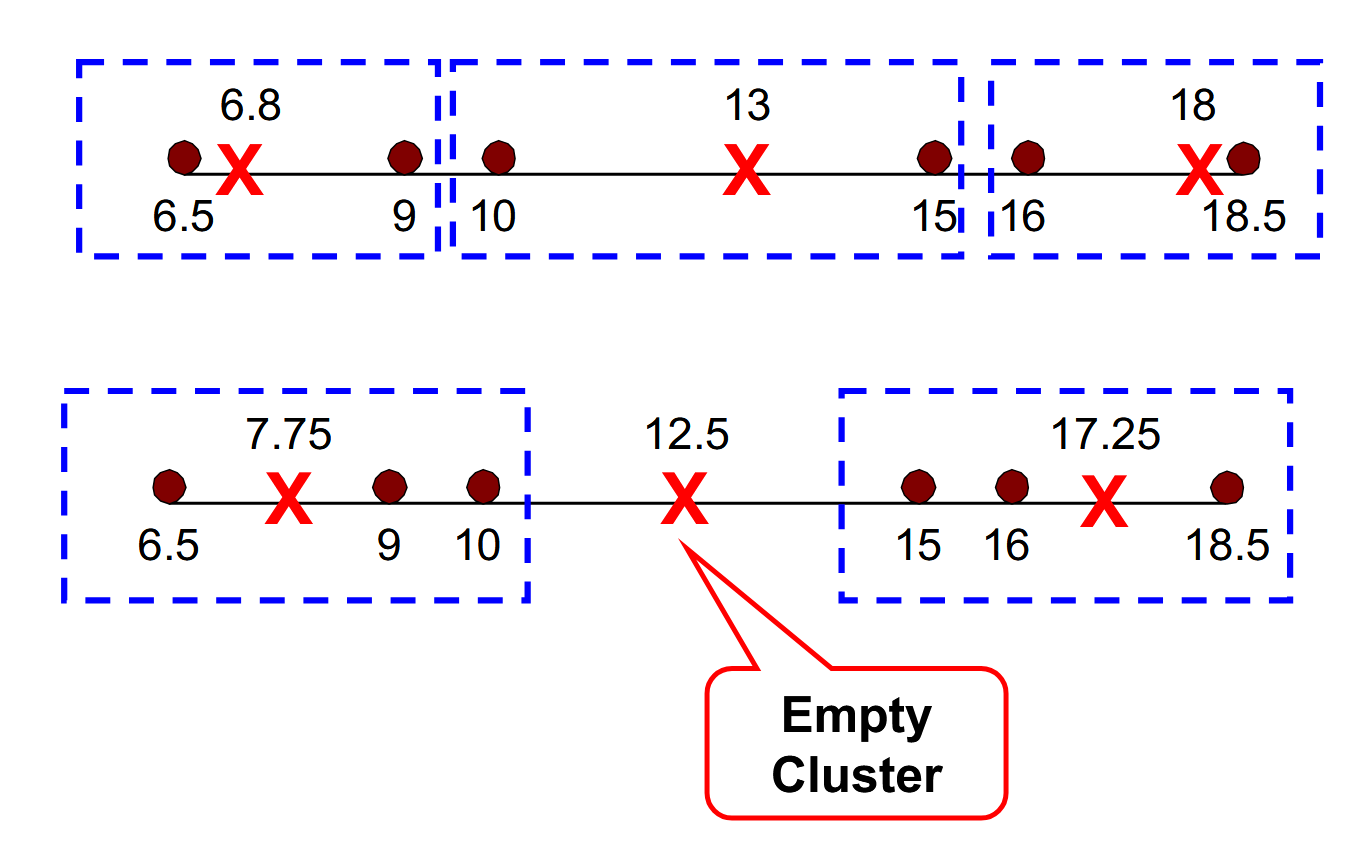
\includegraphics{images/04/kempty.png}
		\caption{K-Means with Empty Clusters}
		\label{fig:04/kempty}
	\end{figure}
\end{paracol}

\subsection{Workflow}
\begin{enumerate}
	\item Data Preprocessing
	      \begin{itemize}
		      \item Handle missing values
		      \item Normalize/standardize data
	      \end{itemize}
	\item Choose the number of clusters $K$
	\item Post processing and validation
	      \begin{itemize}
		      \item Eliminate small clusters that may represent outliers
		      \item Split ‘loose’ clusters, i.e., clusters with relatively high
		            SSE
		      \item Merge clusters that are ‘close’ and that have relatively
		            low SSE
		      \item Can use these steps during the clustering process\\
		            \texttt{ISODATA}
	      \end{itemize}
\end{enumerate}

\subsection{Choosing the number of clusters K}
If there are K ``real'' clusters then the chance of selecting
one centroid from each cluster is small, especially if K is large.

A solution is to run K-Means multiple times with different initial centroids and choose the best result, but probability of getting a good result is still small.

A different approach is to use \textbf{hierarchical clustering} to determine initial centroids for K-Means.

Another option is to \textbf{incrementally} update centroids as points are assigned to clusters, instead of waiting until all points are assigned.
This is more expensive and introduces order dependence.
\nl

We can define a goodness measure of a cluster $c$ (hence of the set of Clusters $C$) as the SSE from the cluster centroid:
\begin{align}
	SSE_C(c,s) &= \sum_{i=1}^{n} (d_i, s_c)^2\\
	G(C,s) &= \sum_{c \in C} SSE_C(c,s)
\end{align}
where $s_c$ is the centroid of cluster $c$, $d_i$ is a point in cluster $c$, and $C$ is the set of clusters.

Re-assignment of points to clusters and re-computation of centroids is guaranteed to \textit{not increase} (or \textit{monotonically decreases}) $G(C,s)$, hence K-Means converges to a local minimum.

At any step we have some value for G(C,s),
\begin{enumerate}
	\item Fix $s$, optimize $C$ $\rightarrow$ Assignment step: assign $d_i$ to the closest centroid $\Rightarrow G(C',s) \leq G(C,s)$
	\item Fix $C'$, optimize $s$ $\rightarrow$ Update step: recompute centroids $\Rightarrow G(C',s') \leq G(C',s) \leq G(C,s)$
\end{enumerate}
In this way the new cost results smaller than the original one, leading to convergence to a local minimum.
\chapter{Diseño de casos de prueba}
\begin{tikzpicture}[node distance=1.5cm]
   \node (model) [rectangle, draw] {Make a model};
   \node (coverage) [rectangle, draw, below of=model] {Pick a coverage criterion};
   \node (testcases) [rectangle, draw, below of=coverage] {Design test cases};

   \draw [->] (model) -- (coverage);
   \draw [->] (coverage) -- (testcases);
\end{tikzpicture}

\section{Modelos}
\note{Recuerda que el SUT (System under test) es el sistema bajo prueba.}

\subsection{Clases de equivalencia}

Se modela el input domain, y para ello se utilizan clases de equivalencia.
Es importante notar que las clases de equivalencia son una asunción, y no una verdad absoluta, pueden ser erróneas.
\begin{paracol}{2}
   
   Sea $R$ una relación de equivalencia sobre un
   conjunto $A$. Para cada $a \in A$, llamaremos
   clase de equivalencia de $a$, al conjunto
   formado por todos los elementos de $A$ que
   estén relacionados con él a través de $R$.
   
   \switchcolumn

   \begin{figure}[htbp]
      \centering
      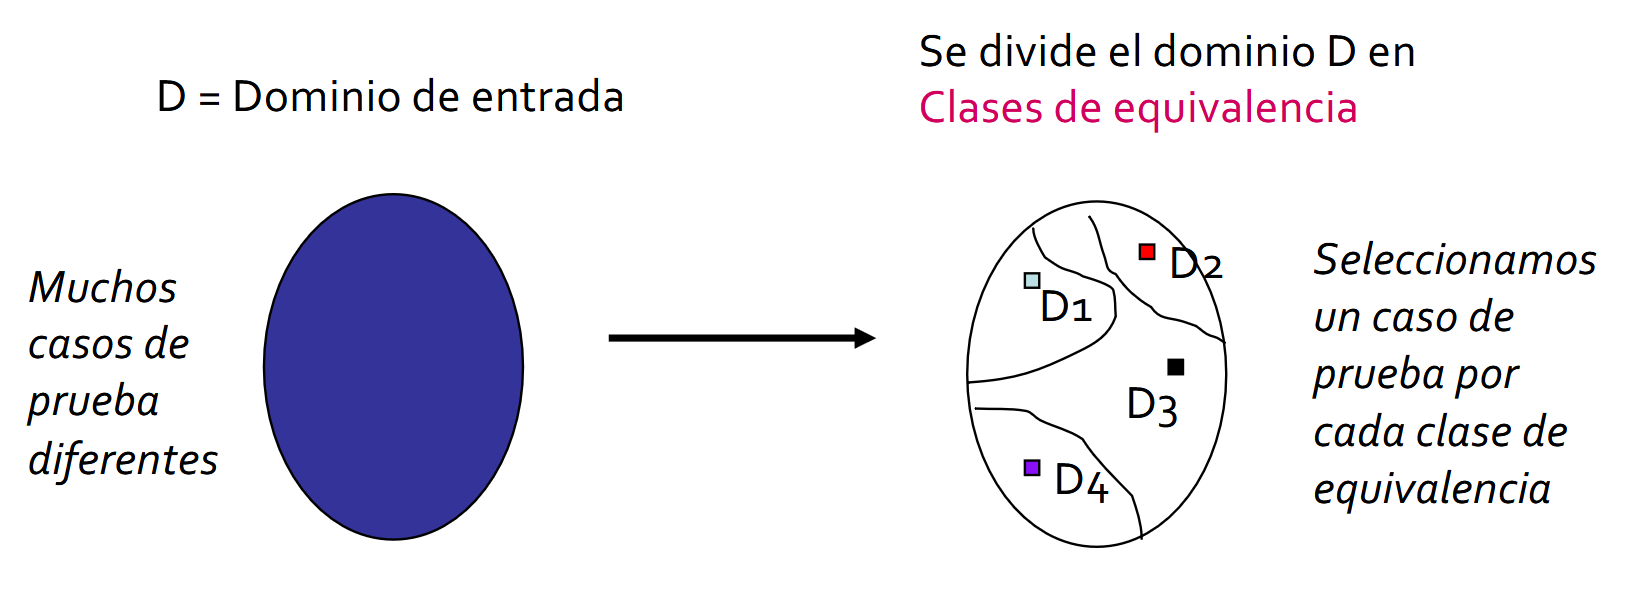
\includegraphics{images/05/claseequivalencia.png}
      \caption{Dividir el dominio}
      \label{fig:05/claseequivalencia}
   \end{figure}
\end{paracol}

Este modelo permite identificar conjuntos de pruebas de tamaño manejable seleccionando unos pocos casos de prueba para cada clase de equivalencia.
Permite también medir la efectividad de la prueba en términos de cobertura relacionada con el modelo de partición creado.
Además, el proceso de partición obliga al tester a pensar sistemáticamente sobre lo que importa

\begin{figure}[htbp]
   \centering
   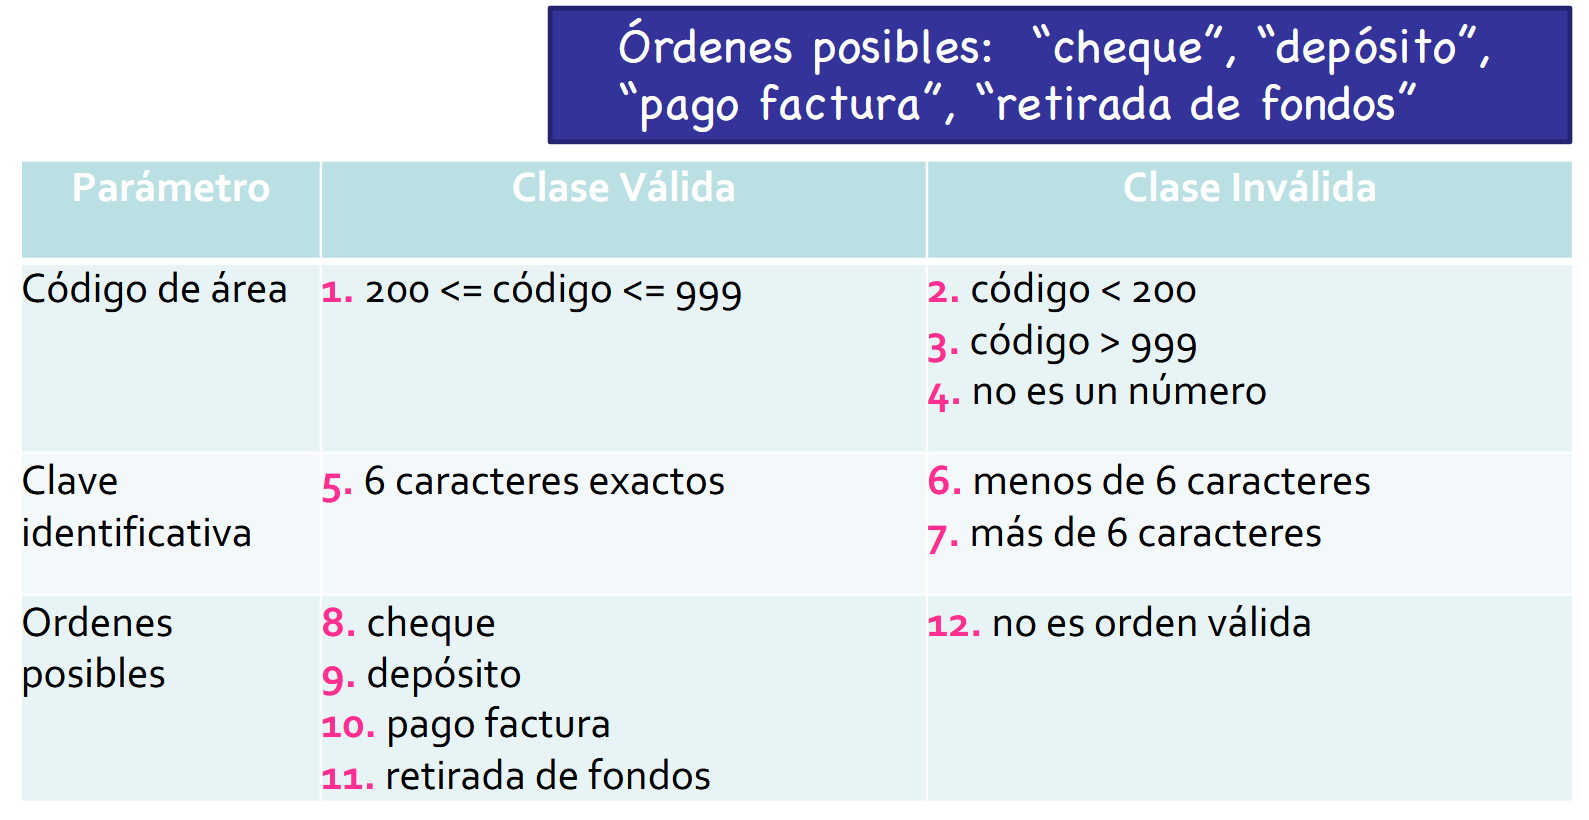
\includegraphics{images/05/claseBanca.png}
   \caption{Ejemplo de una aplicación bancaria}
   {Los datos de entrada son:\ns
   \begin{itemize}
   	\item Código de area: número de tres dígitos que no empieza ni por 0 ni por 1
	\item Clave identificativa de la operación: 6 caracteres alfanuméricos
	\item Órdenes posibles: ``cheque'', ``depósito'', ``pago factura'' , ``retirada de fondos'' 
   \end{itemize}}
   \label{fig:05/claseBanca}
\end{figure}

Es importante enumerar las clases de equivalencia, y no mezclarlas sobre todo.
Cuando se va a escribir las pruebas, cada prueba tiene que ser relacionada con una o más clases de equivalencia, y tenemos que indicar a cuales.

\begin{table}[htbp]
   \centering
   \begin{tabular}{|c|c|c|}
   \hline
       Parámetro & Clase Válida & Clase Inválida \\ \hline
       Capital & $c > min$ & $c \leq min$ \\ \hline
       Ingreso & $i \geq 0$ & $i < 0$ \\ \hline
       Deuda & $d \geq 0$ & $d < 0$ \\ \hline
       Impagados & $T \vee F$ & \\ \hline
       \multirow{4}{*}{Impagados $\wedge$ cond} & 1) $T \wedge (i - d) < c/3$  & ~ \\
       & 2) $F \wedge (i - d) \geq c/3$ & \\
       & 3) $T \wedge (i - d) \geq c/3$ & \\
       & 4) $F \wedge (i - d) < c/3$ & \\ \hline
   \end{tabular}
   \caption{Ejemplo de clases de equivalencia para una aplicación bancaria}
   \note{
   \begin{itemize}
   	\item si el cliente está en una lista de impagados y el sueldo bruto menos la deuda
   	      es inferior al capital solicitado dividido entre 3, la solicitud pasa a No
   	      Concedida.
   	\item si el cliente no está en ninguna lista, y el sueldo bruto menos la deuda es
   	      mayor o igual al capital solicitado dividido entre 3, se clasifica como Pre-
   	      concedida.
   	\item en cualquier otro caso pasa a En estudio
   \end{itemize}
   }
   \label{tab:05/claseEquivalencia}
\end{table}

\section{Tablas de decisión}

Se puede utilizar para programas que toman decisiones basadas en condiciones lógicas sobre combinaciones de entradas, parámetros y/o variables, eligiendo diferentes acciones o respuestas.
\note{\begin{itemize}
	\item La acción o respuesta que se toma no depende del orden en que
se evalúa los valores de los parámetros y variables.
	\item La acción o respuesta que se toma no depende de entradas o
salidas anteriores
\end{itemize}}

\begin{paracol}{2}
   \begin{itemize}
   	\item Cada condición corresponde a una variable, relación o predicado
	\item Valores posibles para las ``Condition Entries''
 \begin{itemize}
 	\item Booleano (\lstinline|True / False|) - Tabla de decisión de entrada limitada
	\item Valores - Tabla de decisión de entrada extendida
	\item Valor ``No Importa'' (Don't care value)

 \end{itemize}
\item Cada acción es una operación que hay que ejecutar

   \end{itemize}
\switchcolumn
\begin{figure}[htbp]
   \centering
   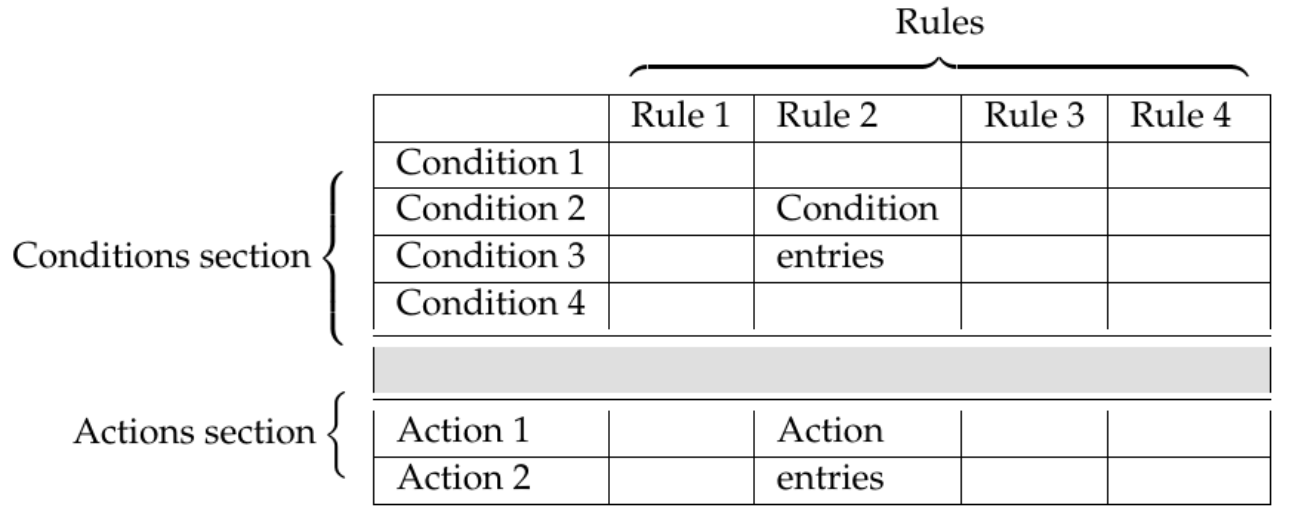
\includegraphics{images/05/tabladecision.png}
   \caption{Tabla decision }
   \label{fig:05/tabladecision}
\end{figure}
\end{paracol}

\begin{figure}[htbp]
   \centering
   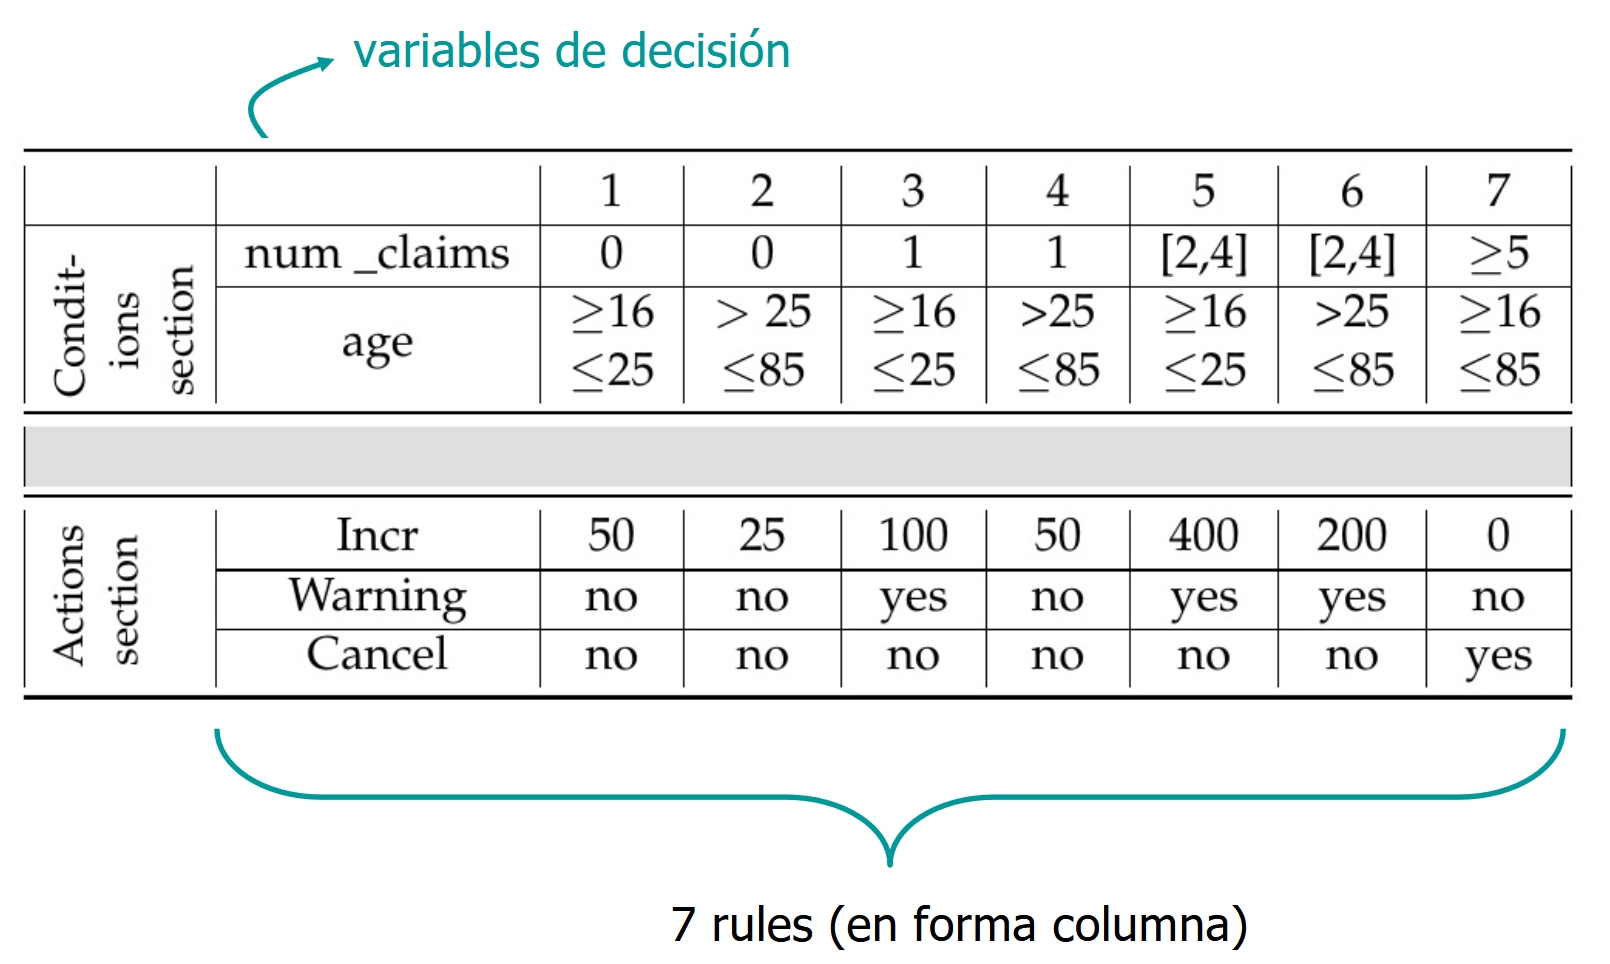
\includegraphics{images/05/tablaForma1.png}
   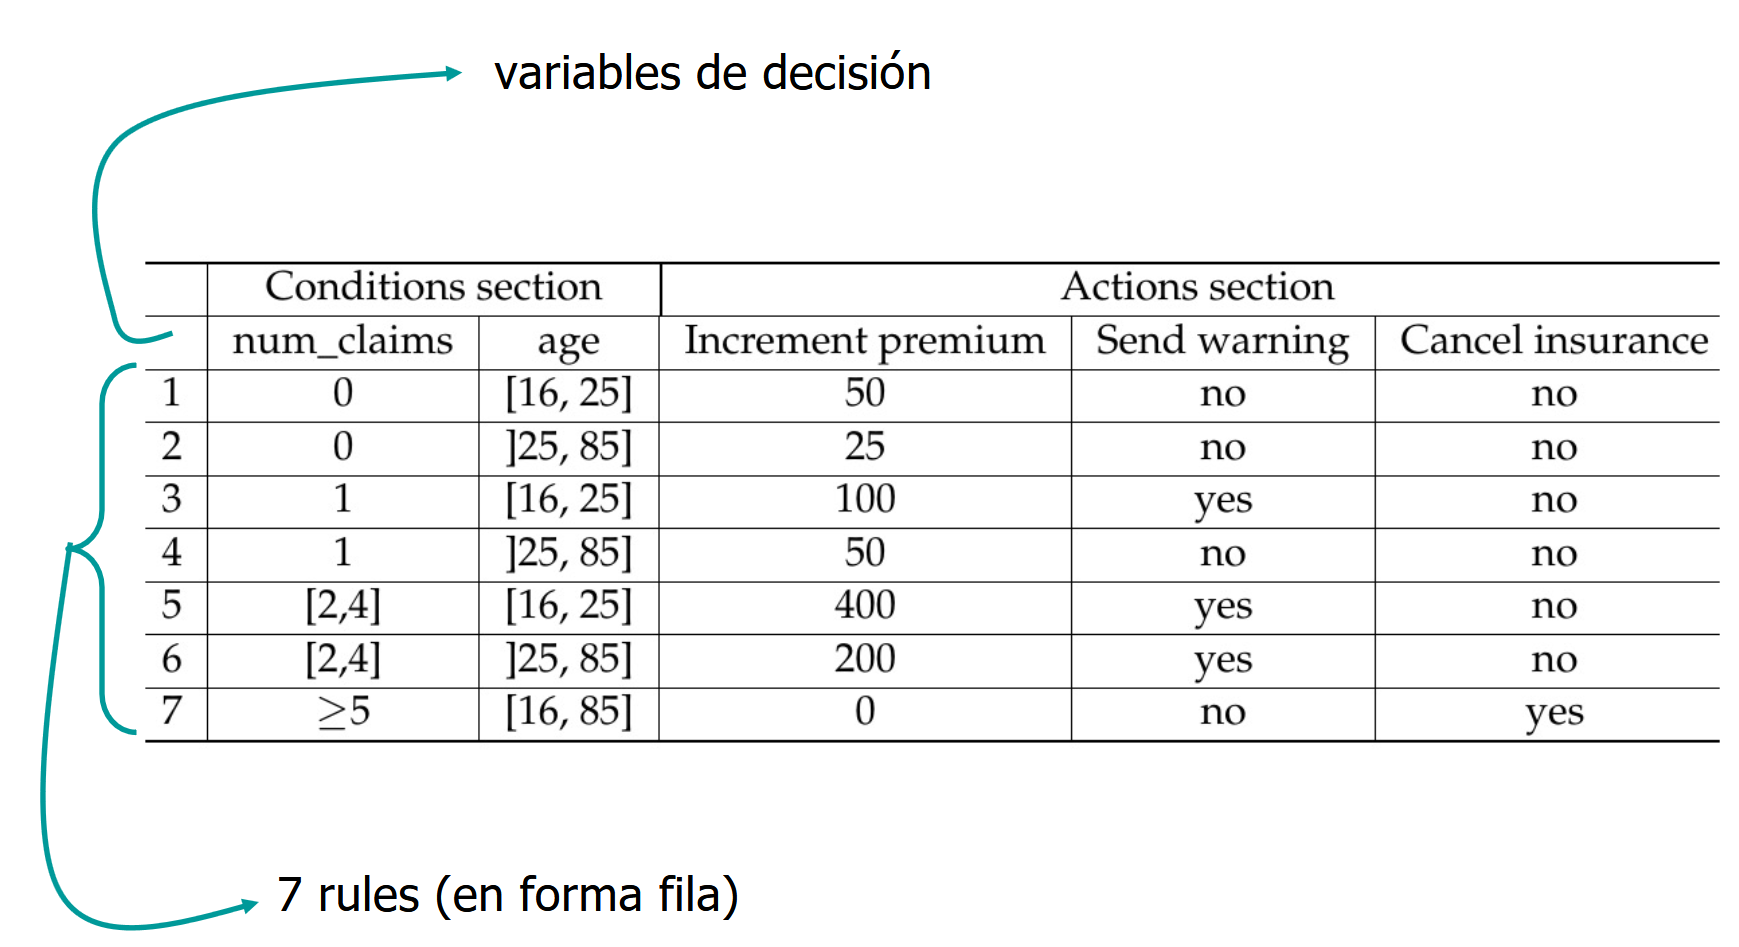
\includegraphics{images/05/tablaForma2.png}
   \caption{Forma columna y forma fila de tablas de decisión}
   \label{fig:05/tablaForma}
\end{figure}

\section{Valores Límites}
\begin{itemize}
	\item Intervalo: un subconjunto del espacio de los valores de entrada de
un programa.
	\item Punto límite de un intervalo (boundary) : aquel punto que según
sea incrementado o decrementado un valor epsilon infinitesimal
dará como resultado un valor perteneciente o no a dicho intervalo.
	\item Desigualdad del límite : una expresión algebraica con $>$, $<$, $\geq$, $\leq$
que define parte de los puntos que pertenecen a un intervalo o
dominio.
	\item Condiciones de igualdad : una expresión algebraica con $=$, $\neq$
\end{itemize}

\begin{figure}[htbp]
   \centering
   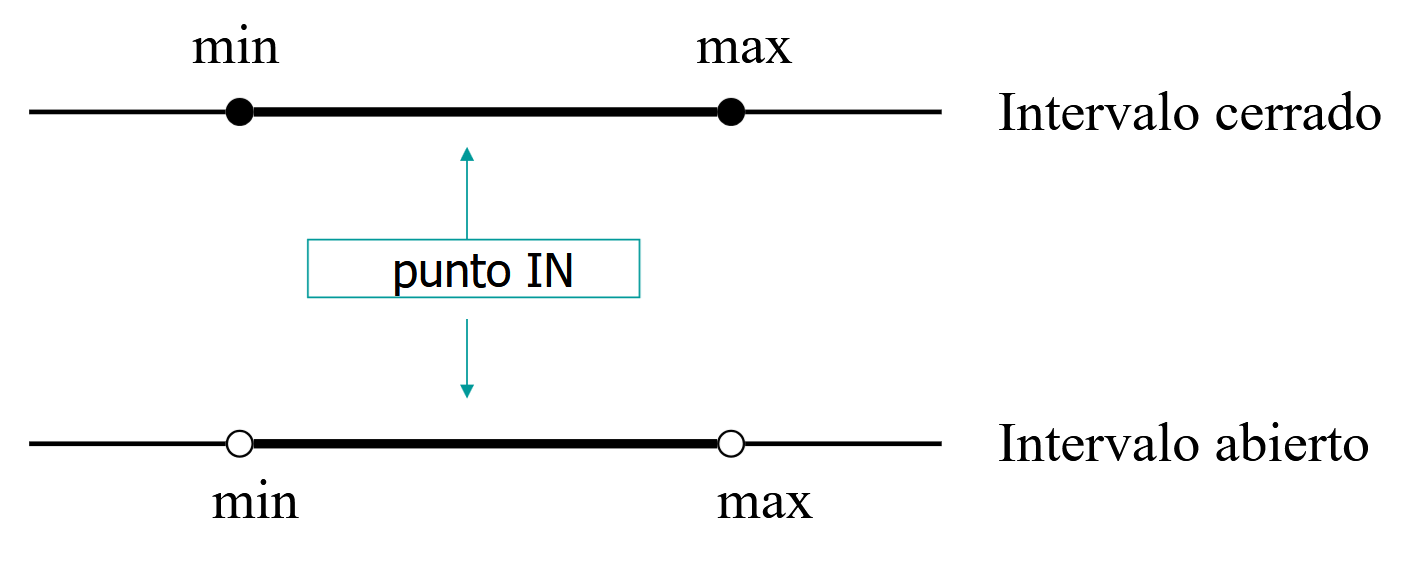
\includegraphics[width=0.45\columnwidth]{images/05/puntoIN.png}
   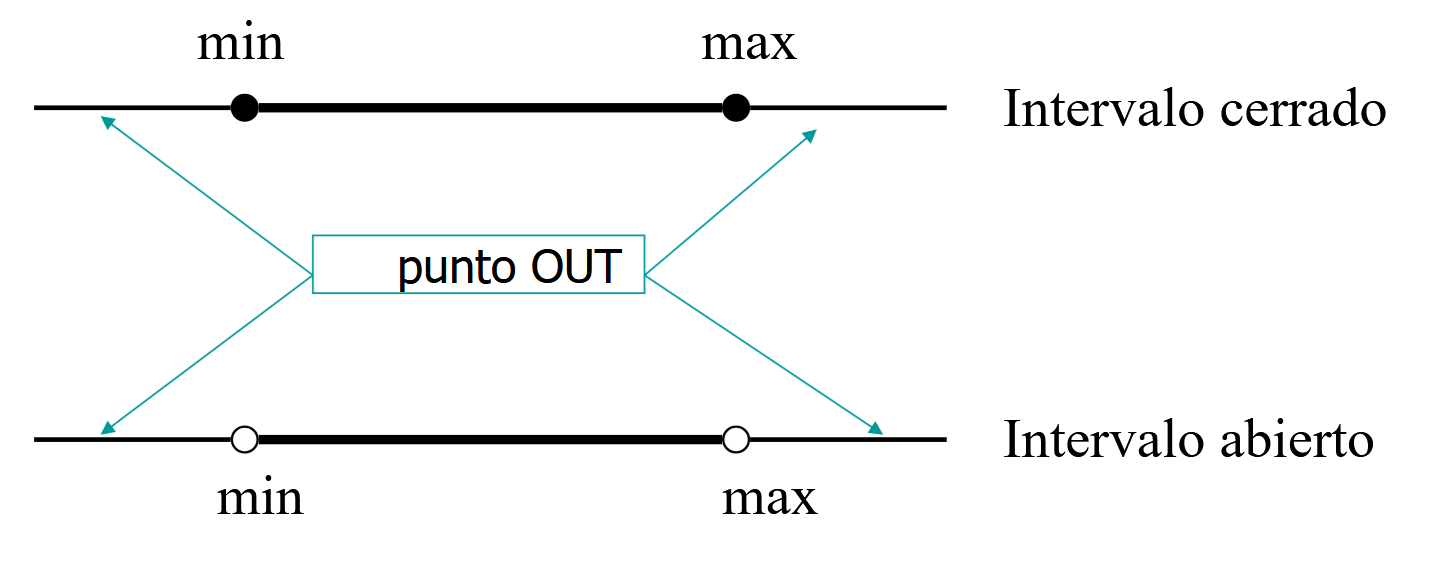
\includegraphics[width=0.45\columnwidth]{images/05/puntoOUT.png}
   \caption{puntoINOUT}
   \label{fig:05/puntoINOUT}
\end{figure}
\begin{figure}[htbp]
   \centering
   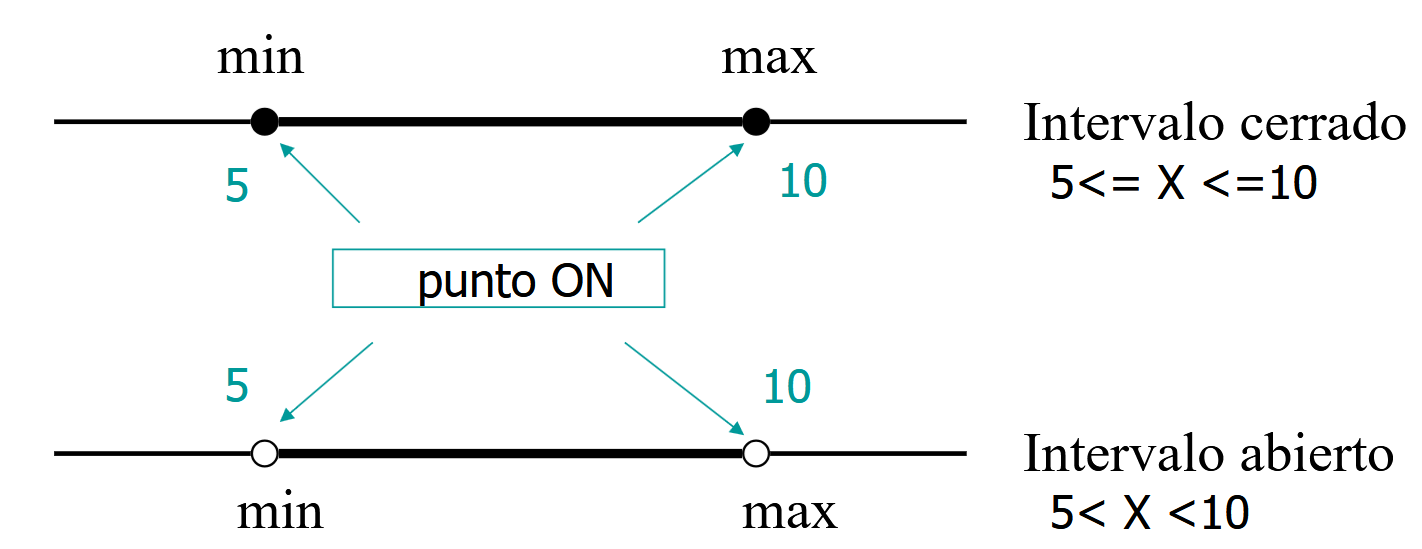
\includegraphics[width=0.45\columnwidth]{images/05/puntoON.png}
   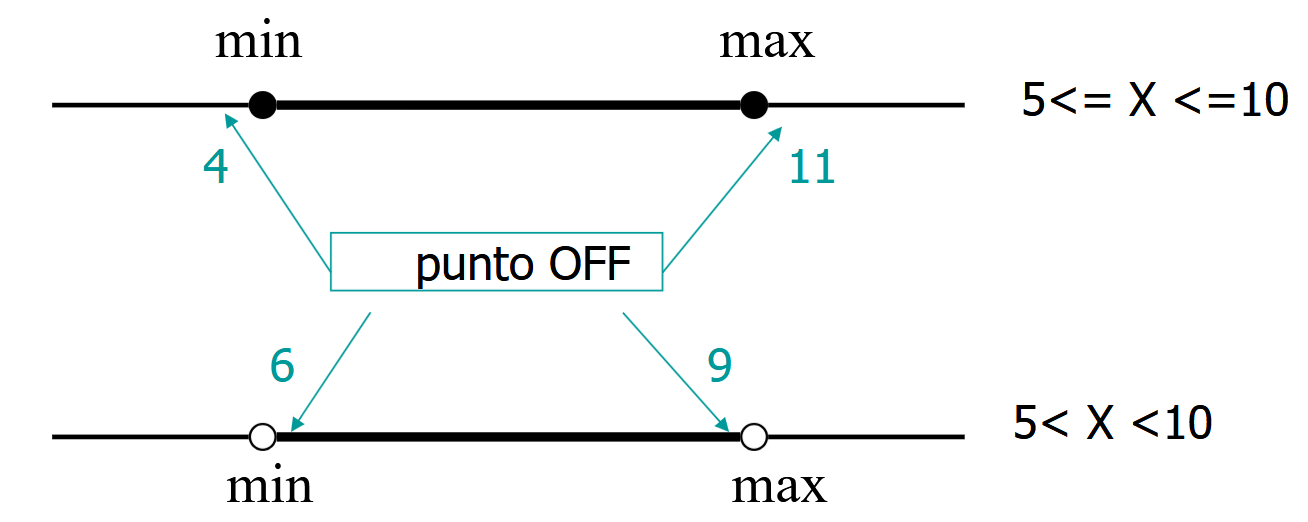
\includegraphics[width=0.45\columnwidth]{images/05/puntoOFF.png}
   \caption{puntoONOFF}
   \label{fig:05/puntoONOFF}
\end{figure}

\begin{itemize}
   \item \textsc{Punto IN} : un punto que pertenece al intervalo
   \item \textsc{Punto OUT} : un punto que no pertenece al intervalo
   \item \textsc{Punto ON} : un punto que pertenece al intervalo y es un límite
   \item \textsc{Punto OFF} : un valor cerca del punto límite de un intervalo
\end{itemize}

La estrategia para diseñar las pruebas de valores límites es 1 punto ON + 1 punto OFF para cada desigualdad de límite.
\note{Ejemplos:
\begin{itemize}
	\item 3 <= extras < 10
	      \begin{itemize}
		      \item Puntos ON: extras = 3; extras = 10
		      \item Puntos OFF: extras = 2; extras = 9
	      \end{itemize}
	\item 2000 < precio\_base <= 5000
	      \begin{itemize}
		      \item Puntos ON?
		      \item Puntos OFF?
	      \end{itemize}
\end{itemize}}


\chapter{Self-stabilization}

\section{Self-stabilization}
In a distributed system a large number of systems are widely distributed and frequently communicate, so there is a chance to end up in an \textbf{illegitimate} state in case, for instance, a message is lost.\\
Among the previously mentioned algorithm and scenarios, consider \textit{token-based} systems: what if the token is lost? Drama \frownie

\note{Note that the meaning of \textit{illegitimate} and \textit{legitimate} depends on the application.}


\begin{definition}
   [Self-stabilization]
   Regardless of the initial state, the system is guaranteed to converge to a legitimate state in a \textbf{finite} number of steps by itself \textbf{without} any \textbf{outside intervention}.
\end{definition}

\subsection{Challenges}
The main challenge in self-stabilization is that nodes in a distributed system do not have a \textit{global memory} that they can access instantaneously.
Each node has to rely on local knowledge and messages from neighbors to make decisions, but their actions must achieve a \textit{global objective}.

\section{System Model}
A Distributed system (DS) model comprises a set of $n$ machines called \textit{processors} that communicate with each other.
\begin{itemize}
   \item Denote the $i^{th}$ processor in the system by $P_i$.
   \item Neighbors of a processor are processors that are \textit{directly} connected to it.
   \item Neighbors communicate by sending and receiving messages.
   \item DS is a \textbf{graph} in which each processor is represented by a node and every pair of neighbouring nodes are connected by link.
   \item FIFO queues are used to model channels for asynchronous delivery of messages: $Q_{ij}$ contains all messages sent by a processor $P_i$ to its neighbor $P_j$ that have not yet been received.
   \item \ul{Each processor is characterized by its state}.
   \item A full description of a DS at a particular time consists of the state of every processor and the content of every queue.
\end{itemize}
Note that this model is quite simplistic. In reality messages are almost \textit{never} delivered in FIFO order: \ul{communications over networks are unpredictable and unreliable}.

\subsection{System Configuration}
The term \textbf{system configuration} is used to describe a DS.
A configuration is denoted by $c = {s_1,s_2,\ldots,s_n,q_{1,2},q_{1,3},\ldots,q_{n,n-1}}$ where $s_i$ is the state of processor $P_i$ and $q_{i,j}$ ($i \neq j$) is the content of the queue from $P_i$ to $P_j$.

\subsection{Network Assumptions}
\begin{itemize}
   \item Let $N$ be an upper bound on $n$ (the number of processors).
   \note{$N$ is important because we may consider dynamic systems}
   \item Let $\gamma$ denote the \textbf{diameter} of the network, i.e., the maximum number of links in any path between any pair of processors.
   \note{Knowing the diameter may provide a bound on the number of hops required for a message to reach any processor from any other processor, ultimately giving a rough upper bound for latency.}
   \item A network is \textbf{static} if the communication topology remains fixed. It is dynamic if links and network nodes can go down and recover later.
   \item In the context of dynamic systems, self-stabilization refers to the time after the “final” link or node failure. The
   term “final failure” is typical in the literature on self-stabilization
   \item Since stabilization is only guaranteed eventually, the assumption that faults eventually stop to occur implies
   that there are no faults in the system for “sufficiently long period” for the system to stabilize.
   \item In any case, it is assumed that the topology remains connected, i.e., there exists a path between any two
   nodes.
\end{itemize}

\section{Self-stabilizing formally said}
We define self-stabilization for a system $S$ with respect to a predicate $P$ over its set of global states, where $P$ is intended to identify its correct execution.

States satisfying $P$ are called \textbf{legitimate} (safe) states, and those that do not are called \textbf{illegitimate} (unsafe) states.

A system $P$ is self-stabilizing with respect to predicate $P$ if it satisfies the following two properties:

\begin{enumerate}
	\item Closure $P$ is closed under the execution of $S$, that is, once $P$ is established in $S$, it cannot be falsified.
	\item \textbf{Convergence} starting from an arbitrary global state, $S$ is guaranteed to reach a global state satisfying $P$ within a finite number of state transitions.

\end{enumerate}

\subsection{Issues in the design of self-stabilizing systems}
Some of the main issues are:
\begin{itemize}
   \item Number of states in each of the individual units in a distributed systems
   \item Uniform and non-uniform algorithms in distributed systems
   \item Central and distribution uniform
   \item Reducing the number of states in a token ring
   \item Shared memory models Mutual exclusion 
   \item Costs of self-stabilization
\end{itemize}

\subsection{Dijkstra's Token Ring Algorithm}
His system consisted of a set of $n$ finite-state machines connected in the form of a \textbf{ring}.

\ul{He defines a \textit{privilege} of a machine as the ability to change its current state}.
This ability is based on a boolean preicate that consists of its current state and the states of its neighbors.

When a machine has a privilege it is able to change its current state, which is referred to as a \textbf{move}.\\
Furthermore, when multiple machines enjoy a privilege at the same time, the choice of the machine that is entitled to make a move is made by a central daemon, which arbitrarily decides the order which privileged machine is allowed to move.

A legitimate state must satisfy the following constraints:
\begin{enumerate}
   \item There must be at least one privilege in the system (liveness, no deadlock).
   \item Every from move from a legal state must again put the system into a legal state (closure).
   \item During an infinite execution, each machine should enjoy a privilege an infinite number of times (no starvation).
   \item Given any two legal states, there is a series of moves that change one legal state to the other (reachability).
\end{enumerate}

Dijkstra considered a legitimate (or legal) state as one in which exactly one machine enjoys the privilege.
\begin{itemize}
	\item This corresponds to a form of mutual exclusion, because the privileged process is the only process that is
allowed in its critical section.
	\item Once the process leaves the critical section, it passes the privilege to one of its neighbours.
\end{itemize}
With this background, let us see how the above issues affect the design of a self-
stabilization algorithm.


\subsection{First Solution}

Machine 0 is exceptional, and the other machines are identical.
% // TODO

\subsection{Second Solution}
We can improve the first solution.

The second solution uses only three state machines ${0,1,2}$.
In the first solution there is only one exceptional machine, the one with state 0.
Here, the machines with state 0 and n-1 are exceptional, the former referred to as bottom machine, the second as top machine.

\begin{itemize}
   \item \textbf{Bottom} machine
   \begin{lstlisting}
      if (S+1) mod 3 == R then
         S := (S-1) mod 3 
   \end{lstlisting}
   \item \textbf{Top} machine
   \begin{lstlisting}
      if L == R and (L+1) mod 3 != S then
         S := (L+1) mod 3 
   \end{lstlisting}
   \item Other machines
   \begin{lstlisting}
      if (S+1) mod 3 == L then
         S := L
      if (S+1) mod 3 == R then
         S := R
   \end{lstlisting}
\end{itemize}

This schema forces the system to always have at least one privilege, hence to self-stabilize.
Actually the number of privileged machines converges linearly to 1.
% // TODO check


\subsubsection{Observations}

The number of states in each of the the individual units that each machine must have for the self-stabilization is an important issue. Dijkstra offered three solutions for a directed ring with $n$ machines, 0,1, \dots, n-1, each having $K$ states, $K \geq n, K=4, K=3.$

% // TODO

\section{To be or not to be\dots Uniform}
In a distributed system, it is desirable and also possible to have each machine use the same algorithm.
However, to design self-stabilizing systems, it is often necessary to have different machines use different algorithms.
% // TODO

Uniformity may lead to not being able to decide who is entitled to make a move, which may lead to a deadlock.
\nl

Generally, the presence of a central demon is assumed in self-stabilizing systems.
% // TODO



\section{Costs of Self-Stabilization}
Clearly, the aim of the designer of a self-stabilizing system is to reduce the convergence span and the response span.

The Time-complexity measure for self-stabilizing systems is the number of \textbf{rounds}.

% // TODO

\section{Designing Self-Stabilizing Systems}
Self-stabilization is characterized in terms of a ``malicious adversary''  that may disrupt the system.

In case the adversary succeeds, a self-stabilizing system is able to recover from the disruption and return to a legitimate state.
\nl


A common technique is \textbf{layering}, as it happens for internet protocols.
This is thanks to the \textit{transitivity} property of self-stabilization: if a system is self-stabilizing and a subsystem is self-stabilizing, then the composed system is self-stabilizing.\\
If $P \rightarrow Q$ ($P$ stabilizes $Q$) and $Q \rightarrow R$, then $P \rightarrow R$.


\chapter{Cyber-Physical Systems}

\section{Introducción}


\begin{definition}
   [CPS]
   A cyber-physical system is a system of collaborating computational
   elements controlling physical entities
\end{definition}
Cyber-Physical System (CPS) is a generic term for a variety of
control systems, such as SCADA (Supervisory Control and Data
Acquisition) systems, ICSs (Industrial Control Systems), BCSs
(Building Control Systems), and the global electrical smart grid

\begin{definition}
   [CPS - 2]
   A Cyber Physical System (CPS) is a network of interacting and
   collaborating computational elements controlling physical entities,
   including sensors, actuators, control processing units, and
   communication devices
\end{definition}

\begin{definition}
   [CPS - 3]
   CPS are systems used to monitor and control the physical world
\end{definition}

\begin{definition}
   [CPS - 4]
   CPS are IT systems that are integrated into physical world application
\end{definition}

\framedt{Events out of temperatures}{
   Consideremos un escenario en el que se mide la temperatura con un sensor.
   Para saber si la temperatura es alta o baja, se necesita un umbral, lo que se llama un \textbf{valor de referencia}.\\
   Esto permite de comparar la temperatura medida con el valor de referencia y tomar una decisión, como por ejemplo generar una alarma si la temperatura es demasiado alta.
}

\section{Componenetes de CPSs}

CPS tienen vulnerabilidades específicas, porque hay:
\begin{itemize}
	\item Issolation asumption
	\item Increased connectivity
	\item Heterogeneity
	\item Long life cycle of components
	\note{Hay softwares que todavía necesitan Windows XP}
\end{itemize}

\begin{figure}[htbp]
   \centering
   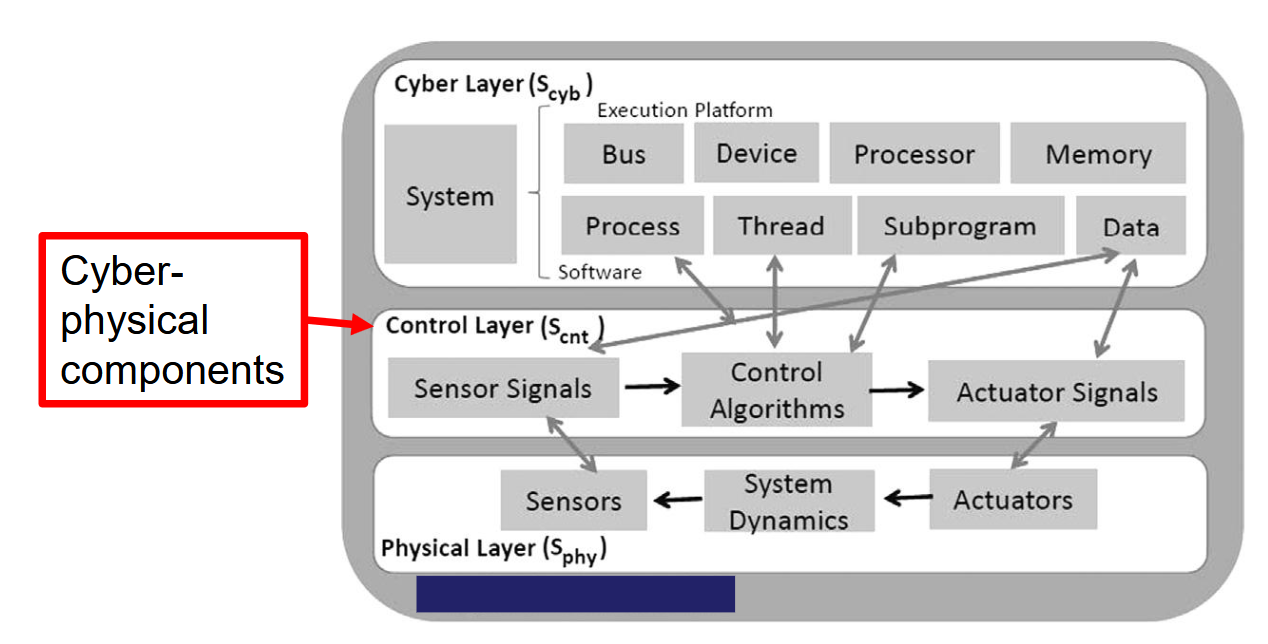
\includegraphics{images/06/CPScomponents.png}
   \caption{Cyberphysical Components}
   \label{fig:06/CPScomponents}
\end{figure}


\subsubsection{Industrial Control Systems}
Sometimes are called SCADA (Supervisory Control and Data Acquisition) systems or DCS (Distributed Control Systems).

El ejemplo más común de ICS son las redes de PLC, por wired o wireless. Tradicionalmente, los PLCs se comunican con un SCADA a través ambos de un protocolo OT (Operational Technologies) de comunicación propietario y de los protocolos IT standard.\\
Tradicionalmente, la isolación era la mejor defensa para estos sistemas.
Patching y updates son un problema, porque los sistemas no pueden ser apagados, y entonces no pueden ser parcheados.

SCADA systems se componen de 4 niveles:
\begin{enumerate}
	\item Sensors and actuators
	\item Distributed controllers, which include programmable logic
   controllers (PLCs), intelligent electronic devices (IEDs), and
   other forms of programmable automation controllers (PACs)
	\item Supervisory and control systems, which encompasses
   systems that store process data, and implements control
   schemes to manage the lower levels
	\item Human machine interfaces (HMIs), which enable the human
   operators to manage the physical process
\end{enumerate}

Diferencias entre ICS y sistemas IT:
\begin{itemize}
	\item Logic execution has a big impact on the physical environtment
	\item Edge devices are, at least, so relevant as hosts servers
	\item Computation resources of edge devices are usually very limited
	\item Safety is the most relevant design constrain
	\item Continuous availability and time-critically constrains
	\item Hard-Real time vs Soft-Real time vs Best-Effort systems
\end{itemize}

SCADA network components:
\begin{itemize}
	\item Servers and workstations that are used by operators to
interact with the field devices segment
	\item HMI software-based graphical user interface
	\item Monitoring of field devices
	\item Field devices data updating
	\item Historian systems
	\item Back up systems (similar to IT systems)
\end{itemize}

Field devices components:
\begin{itemize}
	\item Programmable Logic Controllers (PLCs)
	\item Remote Terminal Units (RTUs)
	\item Intelligent Electronic Devices (IEDs)
	\item IEDs are microprocessor based devices as sensors, motors (actuators),
brakes,lights, etc
	\item IEDs are controled by RTUs and PLCs by mean of field buses
protocols (as PROFIBUS DP)
	\item RTUs monitor IEDs and transmit data to PLCs using ModBUS RTU and
DNP3
	\item Sometimes, directed to the SCADA network using ModBUS TCP
	\item PLCs are control computers, with many types of I/O interfaces
\end{itemize}

Usual incidents in ICSs:
\begin{itemize}
	\item Blocked or delayed flow of information through ICS networks, which could
disrupt ICS operation
	\item Unauthorized changes to instructions, commands, or alarm thresholds, which
could damage, disable, or shut down equipment, create environmental
impacts, and/or endanger human life
	\item Inaccurate information sent to system operators, either to disguise
unauthorized changes, or to cause the operators to initiate inappropriate
actions, which could have various negative effects
	\item ICS software or configuration settings modified, or ICS software infected with
malware, which could have various negative effects
	\item Interference with the operation of equipment protection systems, which could
endanger costly and difficult-to-replace equipment
	\item Interference with the operation of safety systems, which could endanger
human life
\end{itemize}

\section{Vulnerabilidades}
\begin{enumerate}
	\item Vulnerabilities inherent in the CPS product, or platform
vulnerabilities
	\item Vulnerabilities because of poor network design or
configuration, or network equipment vulnerabilities
	\item Vulnerabilities caused during the installation, configuration,
and maintenance of the CPS, or management vulnerabilities
\end{enumerate}

\begin{figure}[htbp]
	\centering
	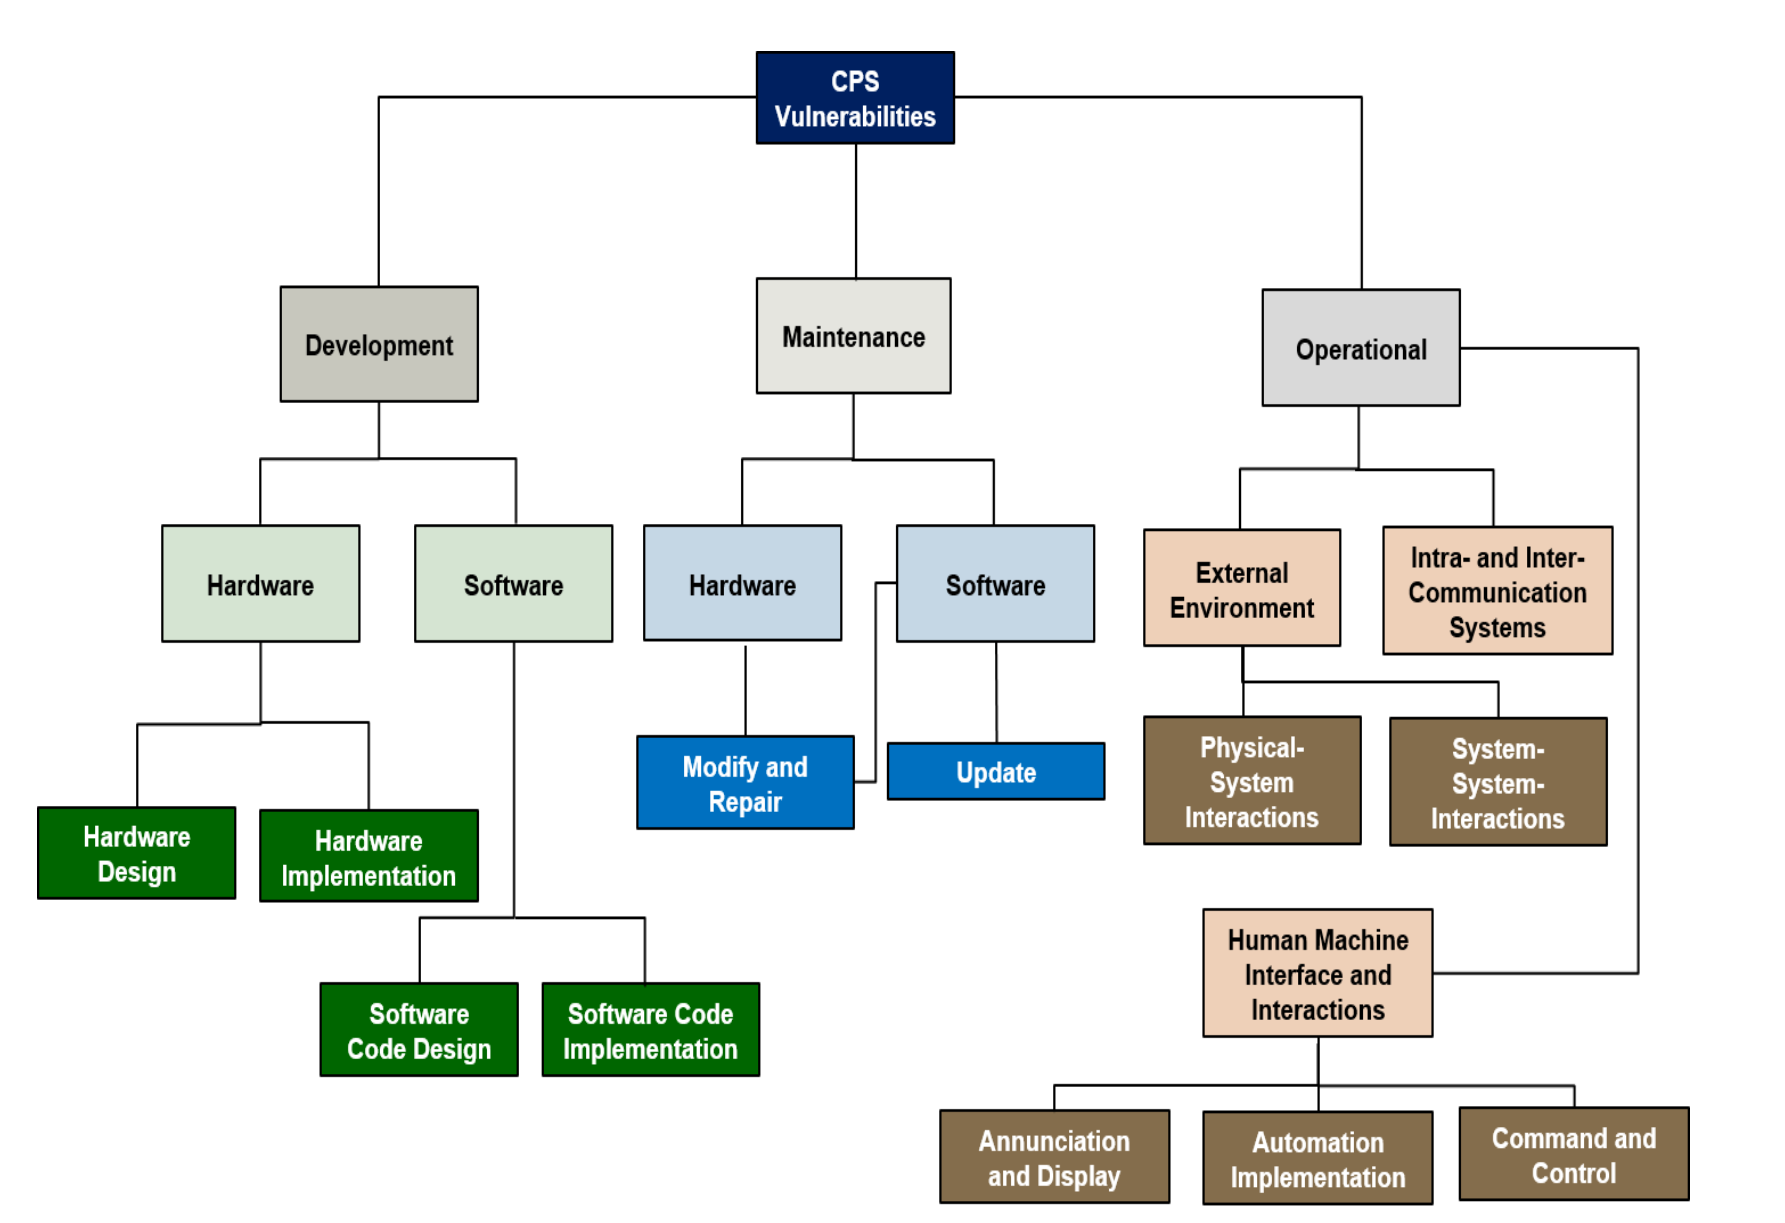
\includegraphics{images/07/cpsVulns.png}
	\caption{CPS Vulnerabilidades taxonomía}
	\label{fig:07/cpsVulns}
\end{figure}

A la izquierda de la figura \ref{fig:07/cpsVulns} hay una lista de vulnerabilidades son vulnerabilidades de plataforma, al centro hay vulnerabilidades de la gestión, y a la derecha vulnerabilidades operacionales.\\
Cómo hemos dicho antes, tipicamente es difícil actualizar el software para CPSs, esto es el motivo por el cual hay muchas vulnerabilidades relacionadas a la mantenimiento del software.

Las vulnerabilidades más comunes son:
\begin{itemize}
	\item Improper Input Validation / Validación incorrecta de las entradas
	\item Permissions, Privileges and Access Control / Permisos, privilegios y control de acceso
	\item Improper Authentication / Autenticación incorrecta
	\item Insufficient Verification of Data Authenticity / Verificación insuficiente de la autenticidad de los datos
	\item Poor Code Quality / Código de baja calidad
	\item Security Configuration and Maintenance / Configuración y mantenimiento de la seguridad
	\item Credentials Management / Gestión de credenciales
\end{itemize}

\subsection{Vulnerabilidades más comunes}
La más explotada vulnerabilidad en CPSs es \textbf{Buffer Overflow}, que es tipicamente permitida por la falta de validación de las entradas: los programadores suelen tener en cuenta lo que debería ocurrir y lo que podría ocurrir por error, pero no todas las posibilidades maliciosas.

Malas prácticas de código permiten a los atacantes suministrar datos inesperados y modificar así la ejecución del programa. Esta vulnerabilidad se llama \textbf{Lack of Bounds Checking}.


\textbf{Cross-Site scripting} vulnerabilidades pueden ser explotadas para muchos tipos de ataques, como el \textbf{Cross-Site Request Forgery} (CSRF), que permite a un atacante ejecutar comandos en el contexto de un usuario autenticado. En general, el Cross-Site Scripting permite \textbf{Code Injection}. 

\section{Vulnerabilities Assessment}
Para los CPS, los objetivos de seguridad están en orden inverso de prioridad, siendo la disponibilidad considerada la más importante, en lugar de la confidencialidad. El personal de la industria a menudo usa el término "seguridad" para referirse a la disponibilidad y fiabilidad del sistema.

Nada debe hacerse en una red CPS activa que pueda interferir o interrumpir las operaciones críticas del sistema. En el entorno CPS, los objetivos de seguridad del mundo IT son reemplazados por la salud y seguridad humana, la disponibilidad del sistema, y la puntualidad e integridad de los datos. Esta es la principal diferencia entre las evaluaciones de seguridad de CPS y de IT.

Esta diferencia también se aplica a las estrategias de mitigación. Ninguna solución de ciberseguridad puede implementarse en la red CPS si interfiere con la respuesta del sistema. El equipo de evaluación cibernética debe trabajar con el personal de la industria y los proveedores para realizar una evaluación efectiva sin comprometer la seguridad, disponibilidad o integridad del CPS.

CPS Vulnerabilities Assessment Execution Phases:
\begin{enumerate}
	\item \textbf{Reconnaissance} -
	The first part of a cyber security assessment is to identify a
target to attack.
	\item \textbf{Exploration} -
	Once a target has been identified, the assessment team attacks
the system
	\item \textbf{Exploit development} -
	Once a problem has been identified, the assessment team may
optionally develop an exploit for the vulnerability.
\item[] All these phases have specific aspects in CPS vulnerabilities assessment
\end{enumerate}

\subsection{Intrusion detection}

HIDS no se utilizan mucho en ICSs, porque ---tipicamente--- no se puede instalar software sobre CPS components.
Entonces, se utilizan \textbf{Network IDS} basados sobre \textbf{anomalias}.
La detección por firmas (signature-based) tiene buena precisión para IT sistemas, pero no lo es para ICSs, porque \dots // TODO

La detección por firmas (signature-based) tiene buena precisión para IT sistemas, pero no lo es para ICSs, porque tiene que depender de firmas conocidas y actualizadas, mientras que los protocolos y comportamientos en entornos ICS son muy específicos y a menudo propietarios.

% \subsection{Lateral Movements}

\textbf{Lateral Movements} son muy comunes en ICSs, porque los atacantes pueden moverse lateralmente a través de la red para obtener acceso a otros sistemas, y entonces, \textbf{honeypots} son una defensa muy eficaz para detectar y monitorear estos movimientos. Los honeypots simulan componentes legítimos del sistema, atrayendo a los atacantes y permitiendo analizar sus técnicas sin comprometer los sistemas reales.

La segmentación de la red, junto con controles de acceso estrictos entre zonas, también es fundamental para limitar la capacidad de los atacantes de moverse lateralmente una vez que han comprometido un punto de entrada inicial en la red ICS.

\subsection{Exploits mitigación}

En general es muy difícil mitigar los exploits en CPSs, porque no se pueden aplicar parches a los sistemas.

% // TODO




\chapter{Raft}


\section{Logs use case}
Before delving into Raft, let's consider an interesting use case. 

Bear in mind that a \ul{\textbf{log} is a \textit{sequence} of records}, it is meaningless if not ordered.
Operations have an effect when executed in an order $s$, and may have a different one in another order $s'$.

In distributed systems, it is not trivial to keep logs consistent.
On local machines, timestamp ordering is enough, but in distributed systems, clocks are not synchronized, hence we need a more sophisticated approach, typically involving the sequencing of operations, not necessarily based on timestamps.

\section{Consesus - (Again)}
Consesus is the backbone of consistency, fault tolerance, and coordination in distributed systems;
it enables systems to operate reliably and predictably, even in the presence of failures and network partitions.

\subsection{Why is it relevant}

\note{\begin{itemize}
	\item \textbf{Coordination}: Synchronizes independent nodes to maintain a consistent state.
	\item \textbf{Fault Tolerance}: Ensures progress and recovery in the presence of failures.
	\item \textbf{Data Integrity}: Prevents data divergence in replicated systems.
	\item \textbf{Avoids Split-Brain}: Manages network partitions to prevent conflicting operations.
	\item \textbf{Strong Consistency}: Guarantees up-to-date data in distributed databases.
	\item \textbf{Leader Election}: Allows seamless transitions of leadership in distributed environments.
	\item \textbf{Transaction Atomicity}: Ensures reliable distributed transactions.
	\item \textbf{State Machine Replication}: Maintains consistent replicated states across systems.
\end{itemize}}

\framedt{Converging}{
   Amongst other things, consesus is used to ensure \textit{\textbf{data integrity}, i.e. prevents \textbf{data divergence} in replicated systems}.
   That is that different data (replicas) will eventually converge to the same value.

   \textit{But to which of the replicas should the others converge?}\\
   Consesus!   

}


\framedt{Paxos and paper}{
   Even though it was a standard until a few years ago, people realized that Paxos was too complex to implement, and could fit best raw paper than actual software.
   Too many aspects were left to the implementer, and it was hard to get it right.
}

\section{Raft}
\ul{Paxos prioritizes safety over liveness}. It guarantees that once a value is chosen, it's always safe, but there may be cases where it fails to make progress quickly.\\
\ul{Raft also ensures safety but uses leader election to optimize for liveness}, making faster decisions when the network conditions allow it.

Raft achieves consesus through an \textit{elected leader} that coordinates the other nodes.
\ul{An entity participating to a Raft cluster can either take the role of the \textbf{leader} or the role of \textbf{follower}};
in the latter case, it may \ul{become leader through a \textit{``candidacy''} process}.\\
{The leader regularly informs the followers of its existence by sending a heartbeat message.\ns
\begin{itemize}
   \item There exist a timeout for the heartbeats from the leader
   \item In case no heartbeat is received the follower changes its status to candidate and starts a leader election.
\end{itemize}}

Note that the \ul{\textbf{underlying assumption} is that \textit{everybody knows everybody}}.

\subsection{Key points}
\begin{itemize}
   \item \textbf{Leader election} - Raft uses a randomized timeout to elect a leader.
   \item \textbf{Log replication} - The leader replicates its log to the followers.
   \item \textbf{Safety and Liveness} - Raft ensures safety and liveness under failure conditions.
\end{itemize}

\subsection{Log Replication}
Log replication is a fundamental mechanism in Raft to ensure that all nodes in the cluster have the same data.

The leader is responsible for replicating its log to the followers. Such log contains a series of commands that must be applied in the same order by all nodes in the cluster.

Only the leader can append entries to the log, and each entry is committed once it is replicated to a majority of the nodes.
\nl

In case the leader crashes it is important to ensure that a new one is elected, and that it has the same log as the previous one.\\
The new leader ensures that the system can continue operating without losing any of the commands already agreed upon by the majority of nodes.

\framedt{Log replication}{
   Log replication is key for ensuring fault tolerance. It guarantees that a log entry is committed when the leader has replicated it to a majority of followers.\\
   Once an entry is committed, it is applied to the state machine on the leader and followers.\\
   This commitment ensures durability: the system guarantees that once a command is applied, it will not be lost, even in the face of failures. 
}

\subsection{Leader election}
There are three states in Raft:
\begin{itemize}
   \item \textbf{Leader} - The leader is responsible for managing the replication of the log.
   \item \textbf{Follower} - The follower replicates the leader's log.
   \item \textbf{Candidate} - The candidate is a node that is trying to become the leader.
\end{itemize}

\framedt{Becoming the leader}{
   \begin{enumerate}
      \item When the current leader fails (e.g. crashes or becomes unreachable), a new leader is elected.
      \item Follower nodes can become candidates and initiate electionss if they don't receive a heartbeat from the leader within a specified time (election timeout).
      \item Leader election is the foundation of Raft's fault tolerance.
   \end{enumerate}
}

Once a leader is elected, the leader appends new log entries and replicates them to all followers.
A log entry is considered committed when it is replicated to a majority of nodes. Followers always accept entries from the current leader to maintain consistency.

\tikzset{every loop/.style={min distance=10mm,in=50,out=490,looseness=10}}
\begin{figure}[htbp]
   \centering
   \begin{tikzpicture}[
      state/.style={rectangle, rounded corners, draw=black, very thick, minimum height=3em, inner sep=3pt, text centered},
      arrow/.style={-{Latex[length=3mm, width=2mm]}, thick},
      every node/.style={font=\sffamily}
  ]
  
  % States
  \node[state] (follower) {Follower};
  \node[state, right=4cm of follower] (candidate) {Candidate};
  \node[state, right=4cm of candidate] (leader) {Leader};
  
  % Arrows
  \draw[arrow] (follower) -- node[above] {Suspects leader failure} (candidate);
  \draw[arrow] (candidate) -- node[above] {win election} (leader);
  \draw[arrow, bend left] (leader) to node[above] {heartbeat timeout} (follower);
  \draw[arrow, bend left] (leader) to node[below] {step down} (follower);
  \draw[arrow, loop above] (candidate) to node[above] {election timeout} (candidate);
  
  \end{tikzpicture}
   \caption{State diagram}
   \label{fig:state_diagram}
\end{figure}

\subsubsection{Ensuring Safety and Liveness}
\proscons{Safety}{Liveness}
   {
    \begin{itemize}
    	\item Raft ensures that the logs of all nodes are consistent. No two nodes will decide on different values, maintaining the consistency property.
    \end{itemize}
   }
   {
    \begin{itemize}
    	\item Raft guarantees that as long as a majority of nodes are functioning, the system will continue to make progress (Liveness). Raft avoids the Liveness issues that Paxos sometimes faces, especially with leader election and split-brain situations
    \end{itemize}
   }

\subsection{Raft Election and Voting process}
\subsubsection{Election}

\begin{itemize}
	\item Election Term and Leader State:
	      \begin{itemize}
		      \item term number represents a logical clock that increases monotonically whenever a new election is initiated.
		      \item prevent conflicts during leader election and ensures a unique identifier for each term.
	      \end{itemize}

	\item Follower State:
	      \begin{itemize}
		      \item When a node starts or after a leader election, it begins in the follower state.

	      \end{itemize}
	\item Candidate state:
	      \begin{itemize}
		      \item If a follower does not receive any communication from the leader within a given timeout, it transitions to the candidate state and starts a new election term.
		      \item The candidate increments its current term number and requests votes from other nodes.
	      \end{itemize}
\end{itemize}

\subsubsection{Voting process}
\begin{itemize}
   \item \textsc{RequestVote}:
   \begin{itemize}
   	\item When a candidate transitions to the candidate state, it sends \textsc{RequestVote} to all other nodes in the cluster.
	   \item \textsc{RequestVote} includes the candidate’s term number, its own last log index and term, and its eligibility for becoming the leader.
   \end{itemize}
   \item Voting process:
   \begin{itemize}
   	\item When a follower receives a \textsc{RequestVote}, it checks if the candidate’s term number is higher than its own.
	   \item If so, it updates its current term and resets its election timeout, acknowledging the leader about the election
   \end{itemize}
   \item Candidate state:
   \begin{itemize}
	   \item if a candidate receives votes from a majority of the nodes in the cluster, it becomes the new leader for the current term.
	   \item If a candidate does not receive enough votes, it returns to the follower state and waits for the next election timeout to start a new election term
   \end{itemize}
   \item Leader state:
   \begin{itemize}
	   \item Upon becoming the leader, the node starts sending \textsc{AppendEntries} to replicate log entries to the followers.
	   \item The leader's election timeout is reset periodically to prevent unnecessary re-elections while it continues to serve as the leader.
   \end{itemize}
   \item Heartbeats:
   \begin{itemize}
      \item The leader regularly sends \textsc{AppendEntries} RPCs with empty log entries (heartbeats) to maintain its authority and prevent other nodes from starting new elections
   \end{itemize}
\end{itemize}

\section{Consensus Takeaways}
\begin{itemize}
	\item Consensus Problem:
	      \begin{itemize}
		      \item Distributed consensus is the challenge of getting a set of distributed nodes (processes) to agree on a single value, despite failures and message delays.
	      \end{itemize}
	\item Importance of Consensus:
	      \begin{itemize}
		      \item Critical for ensuring data consistency and fault tolerance in distributed systems.
		      \item Powers key systems like databases, replicated state machines, and blockchain technologies.
	      \end{itemize}
	\item Key Properties of Consensus:
	      \begin{itemize}
		      \item Safety: The algorithm ensures that nodes never decide on conflicting values. Once a value is decided, it
		            remains fixed.
		      \item Liveness: The system eventually reaches a decision, despite failures or delays, ensuring progress.

	      \end{itemize}
	\item Challenges in Asynchronous Systems:
	      \begin{itemize}
		      \item In asynchronous systems, where nodes can experience delays or crashes, achieving both safety and liveness simultaneously is challenging.
		      \item The FLP Impossibility Theorem proves that no deterministic consensus algorithm can guarantee both safety and liveness in full y asynchronous systems with even a single faulty node.
	      \end{itemize}
	\item Paxos:
	      \begin{itemize}
		      \item A widely used consensus algorithm focused on safety. It guarantees that nodes will agree on a value, but it may fail to make progress in some situations, hence not guaranteeing liveness in every case.
	      \end{itemize}
	\item Raft:
	      \begin{itemize}
		      \item Raft is a consensus algorithm designed for understandability and practicality. It divides the consensus process into two dist inct phases: leader election and log replication.
		      \item Raft guarantees safety by ensuring that only one leader is elected, and achieves liveness under normal conditions, though like Paxos, it may struggle under certain network partitioning scenarios.
		      \item Its straightforward structure and clear separation of roles make it widely adopted in distributed systems that prioritize clarity and
		            maintainability.

	      \end{itemize}
	\item Consensus Mechanisms in Practice:
	      \begin{itemize}
		      \item Consensus algorithms like Paxos and Raft are the backbone of many distributed systems to ensure reliability, consistency, and fault tolerance, from databases to large-scale cloud systems.
	      \end{itemize}
\end{itemize}

\end{document}
